\chapter{Diseño e implementación}
\label{cap:diseno}
En este capítulo se documenta el diseño e implementación que se ha realizado para dar lugar a la aplicación final. Como bien se explica en el capítulo dedicado a la arquitectura, se ha seguido una división por subsistemas por lo que la mejor aproximación para separar ahora los múltiples diagramas de clases es hacerlo por paquetes, asociados cada uno de ellos a un subsistema. Además se generarán una serie de paquetes que contienen una serie de funcionalidades adicionales utilizadas por los otros.

\bigskip

Se empezará por la documentación asociada a los paquetes relacionados con el motor del videojuego en sí mismo para luego seguir con el subsistema de la lógica de la aplicación que contendrá la implementación del agente. Luego se muestran los diagramas de interacción que relacionan las clases antes definidas con los casos de uso en los que participan. Finalmente se mostrará cómo se llegó al diseño de la interfaz gráfica de la aplicación. Además, se ha hecho uso de un \textbf{código de colores} que permite una comprensión más rápida de cada uno de los diagramas:

\begin{itemize}
	\item \textbf{Verde}: Identifica las clases protagonistas o principales de cada diagrama.
	\item \textbf{Morado}: Identifica las clases que ayudan a las principales a realizar la función que se les requiere, estas clases \textbf{pertenecen} al paquete/diagrama que se está mostrando.
	\item \textbf{Amarillo}: Identifica las clases que son necesarias para llevar a cabo las funcionalidades del paquete/subsistema pero que \textbf{no pertenecen} al mismo.
	\item \textbf{Azul}: Identifica las clases, estructuras o enumeraciones que representan contenedores de datos sin funcionalidades complejas.
\end{itemize}

\section{Diagramas de clases}

Para facilitar la comprensión de la estructura de esta sección la misma está ordenada de la siguiente forma:

\begin{enumerate}
	\item Primero se explicará la estructura asociada al bus de mensajes.
	\item Luego se mostrará la estructura genérica de la aplicación con todos los subsistemas.
	\item Se explicarán los subsistemas individualmente.
	\item Brevemente, se mencionarán algunas clases adicionales.
	\item Finalmente se mostrarán los diagramas de cada una de las escenas.
\end{enumerate}

En los apartados que siguen se añadirá una breve explicación asociada a cada diagrama para favorecer su comprensión.  Además, en aras de mantener la simplicidad de los diagramas, se han omitido los constructores que no aportan información sobre la clase, es decir, si una clase no requiere argumentos o requiere los mismos que una superclase no se mostrará su constructor. En situaciones donde sea relevante, como que requiera argumentos inesperados o el constructor sea privado, se especificará como tal.

\subsection{Bus de mensajes}

\begin{figure}
	\centerline{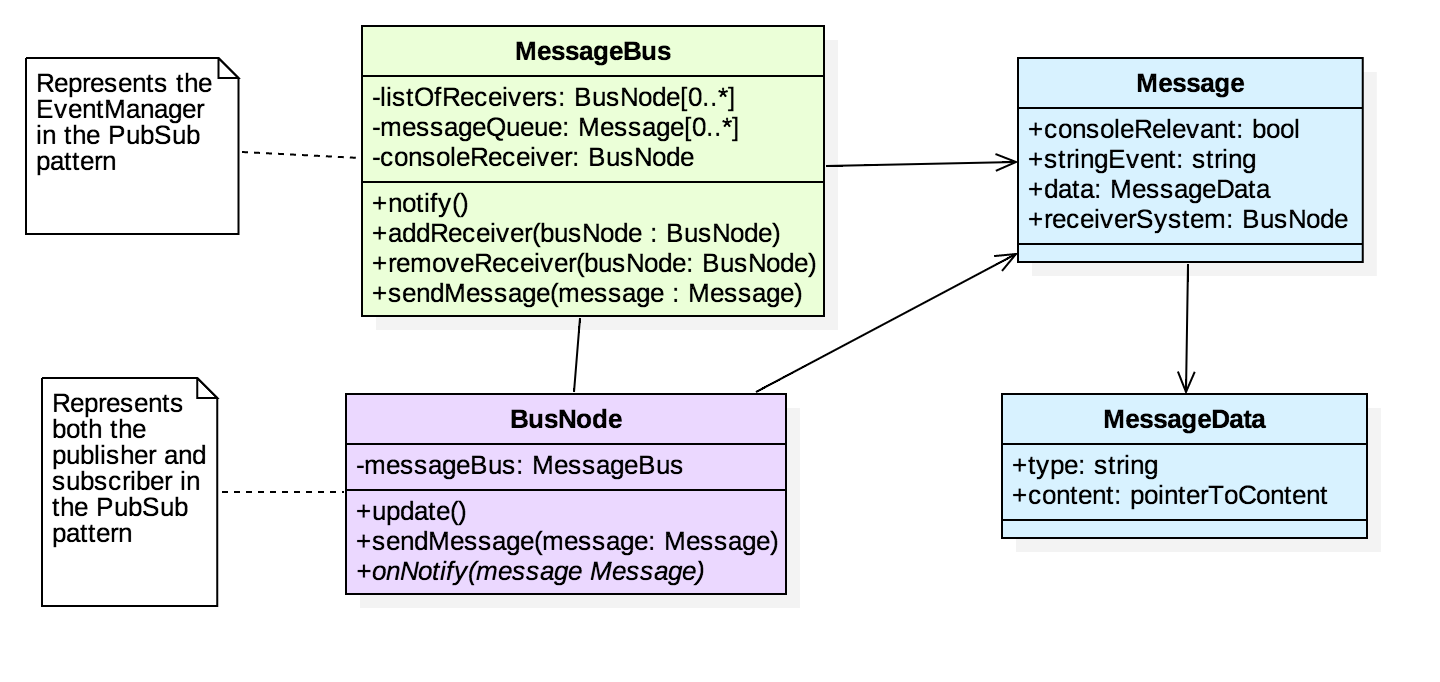
\includegraphics[width=15cm]{otros/UML/png/alld/png/messaging__diagramaDeClases_messaging_11.png}}
	\caption{Diagrama de clases del bus de mensajes}
	\label{class:messageBus}
\end{figure}

En la figura \ref{class:messageBus} se encuentra el diagrama de clases del bus de mensajes, en el mismo se vé implementada una modificación del patrón \textit{PubSub} (mostrado en la figura \ref{pat:pubsub}) en la cual la clase \textbf{\textit{BusNode}} representa tanto a los publicadores como a los subscriptores. Dicha clase es la encargada de encapsular las funcionalidades asociadas a enviar y recibir mensajes por parte de cada subsistema.

\bigskip

Por otra parte, la clase \textbf{\textit{MessageBus}} es la que representa el \textit{EventManager} del patrón \textit{PubSub}. La misma es la encargada de almacenar los mensajes y enviarlos a todas las instancias de \textit{BusNode} que lo requieran.

\bigskip

Finalmente, se ven las clases \textbf{\textit{Message}} y \textbf{\textit{MessageData}} que representan los mensajes que se envía y su contenido.

\subsection{Aplicación general}

\begin{figure}
	\centerline{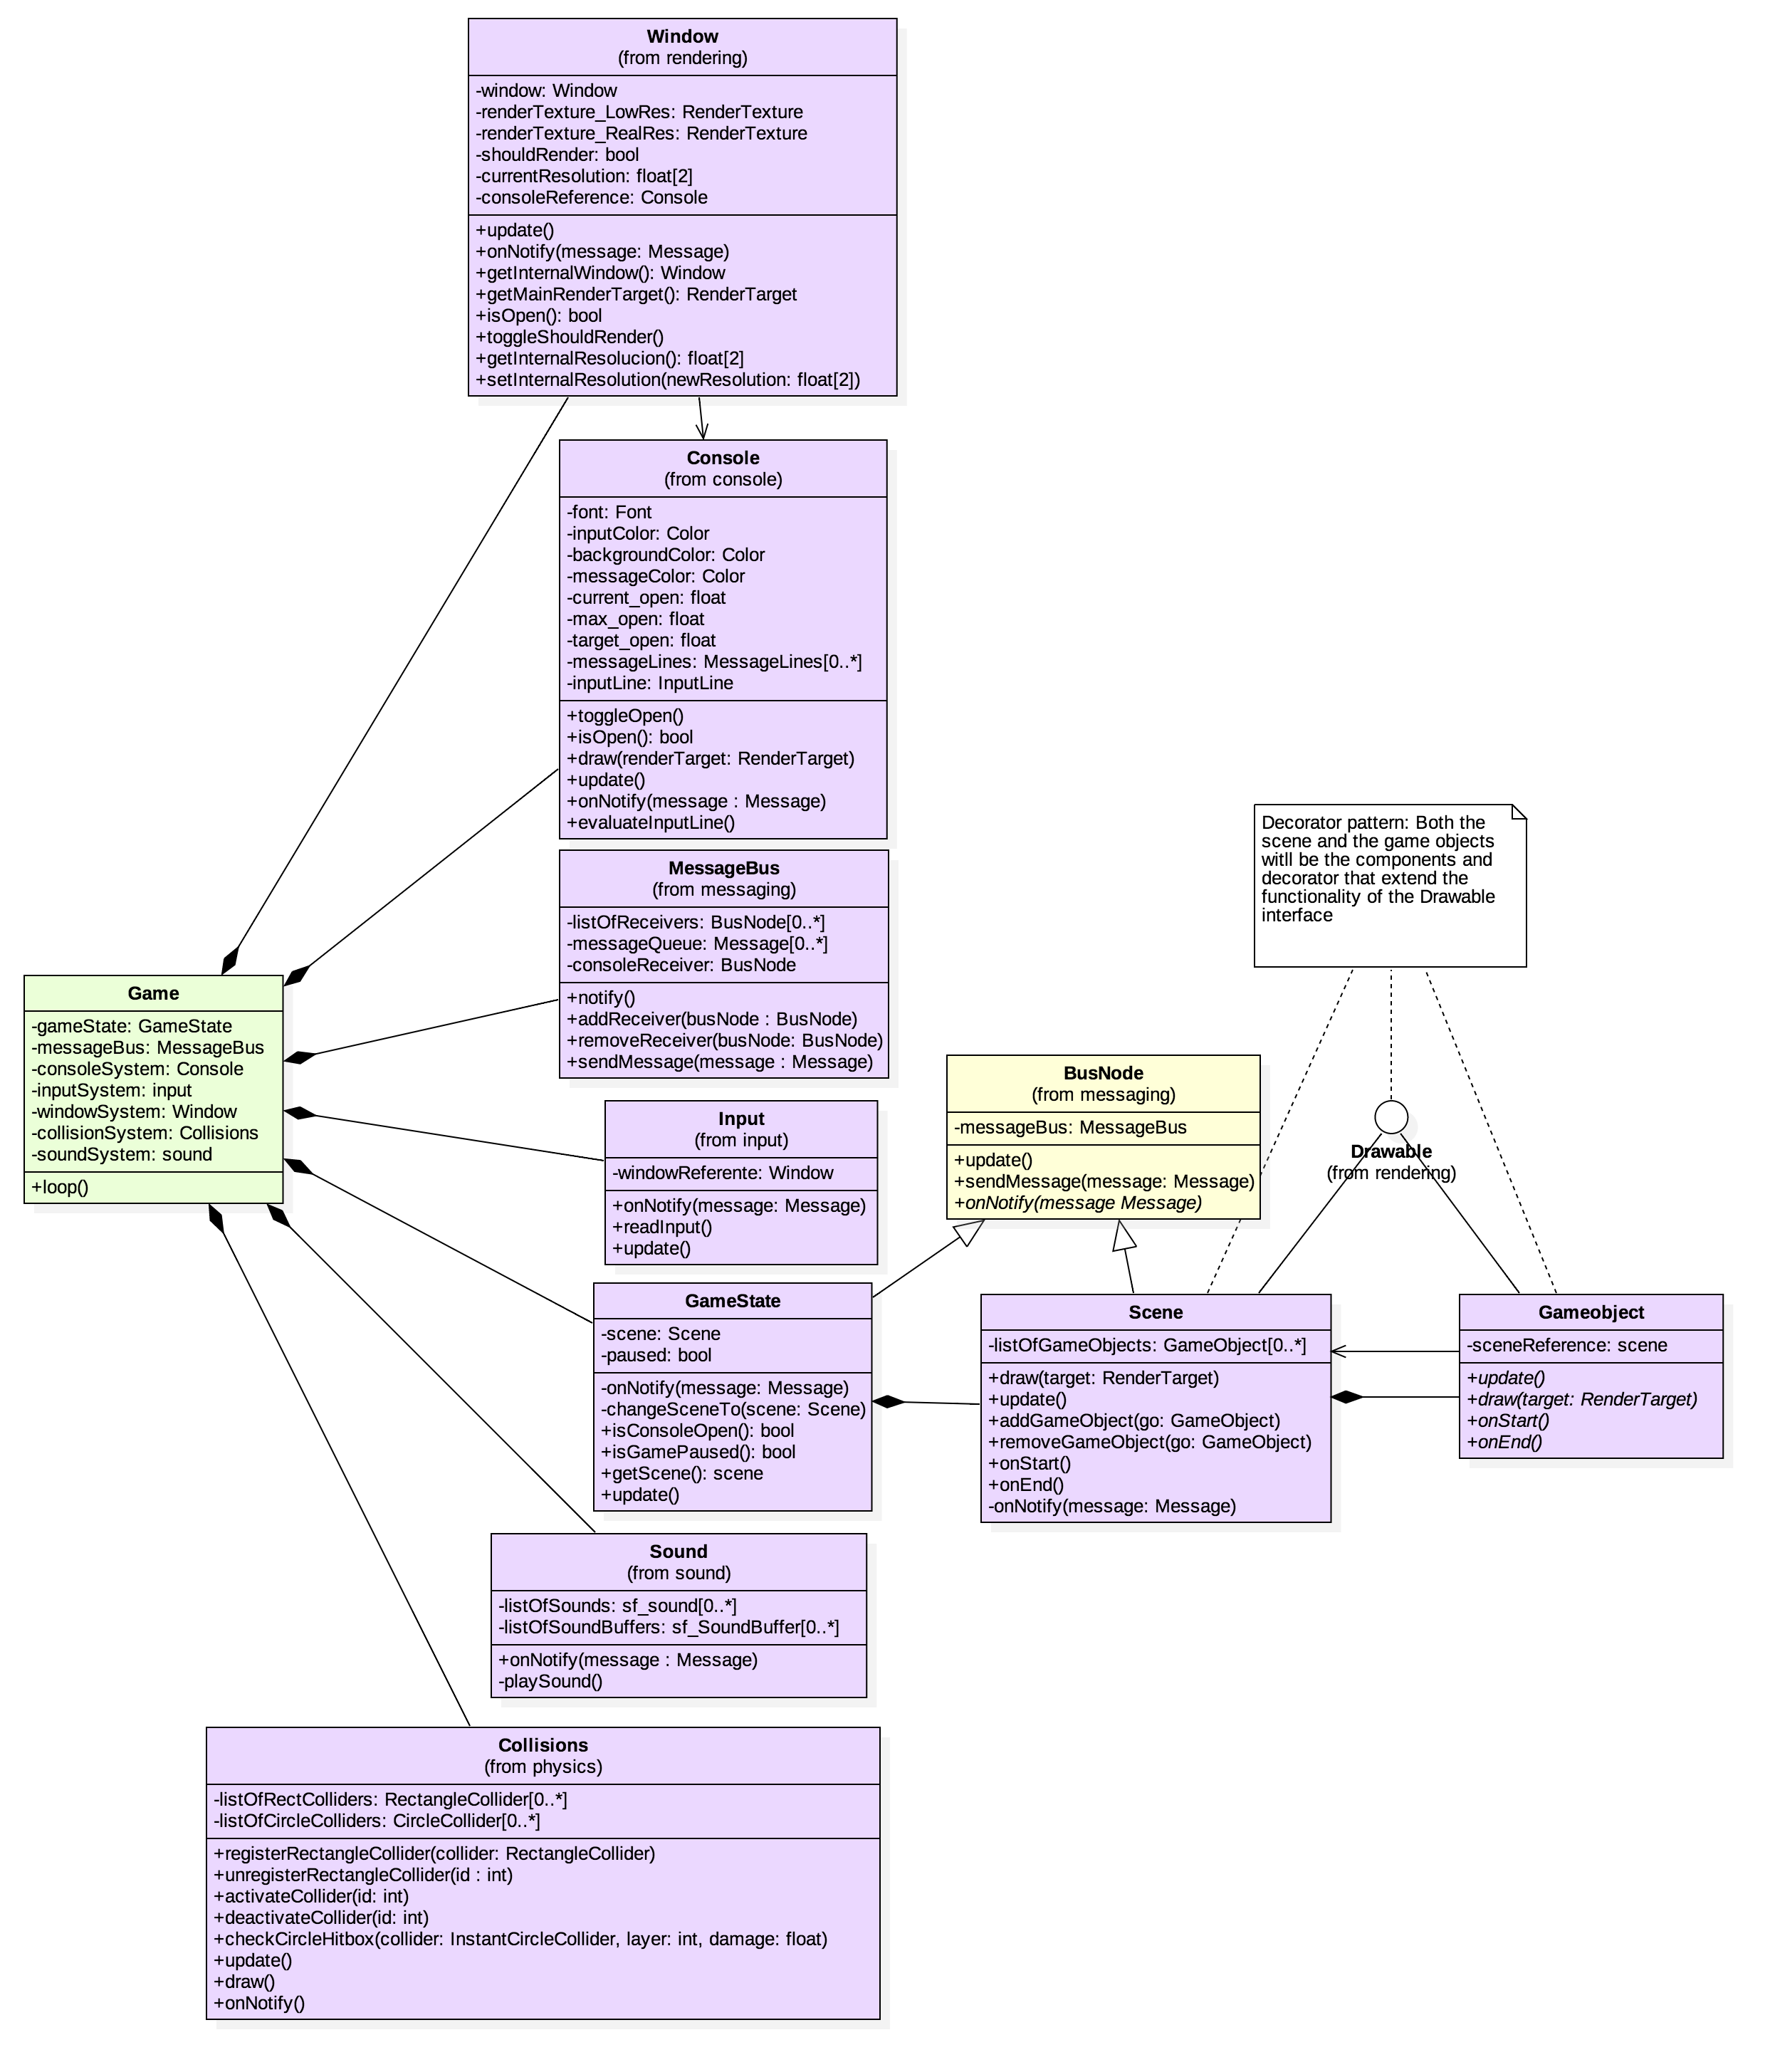
\includegraphics[width=18cm]{otros/UML/png/alld/png/gamelogic__diagramaDeClases_gamelogic_7.png}}
	\caption{Diagrama de clases de la lógica del juego}
	\label{class:gamelogic}
\end{figure}

La figura \ref{class:gamelogic} contiene la lógica del juego mostrada a muy alto nivel. La clase principal es \textbf{\textit{Game}} que es instanciada en el \textit{main} de la aplicación. La misma contiene la función \textit{loop} que simplemente itera por todos los subsistemas, actualizándolos, como se ve en el diagrama de secuencia \ref{sec:general}. 

\bigskip

También se observan las clases asociadas a cada uno de los subsistemas, muy importante es la clase \textbf{\textit{GameState}} que contiene a la escena de la aplicación representada por la clase \textbf{\textit{Scene}}. Aquí podemos ver el patrón \textit{Decorator} (Figura \ref{pat:decorator}) en el cual la escena y los \textit{gameobjects} (representados en la clase \textbf{\textit{GameObject}}) agregan estado y funcionalidad. Cada \textit{gameobject} representa uno de los objetos pertenecientes a la escena desde el punto de vista del juego a alto nivel, esto puede ser un personaje, texto, una barra de vida, un contador de tiempo, etc.


\subsection{Subsistemas}

\subsubsection*{Subsistema de consola}

\begin{figure}
	\centerline{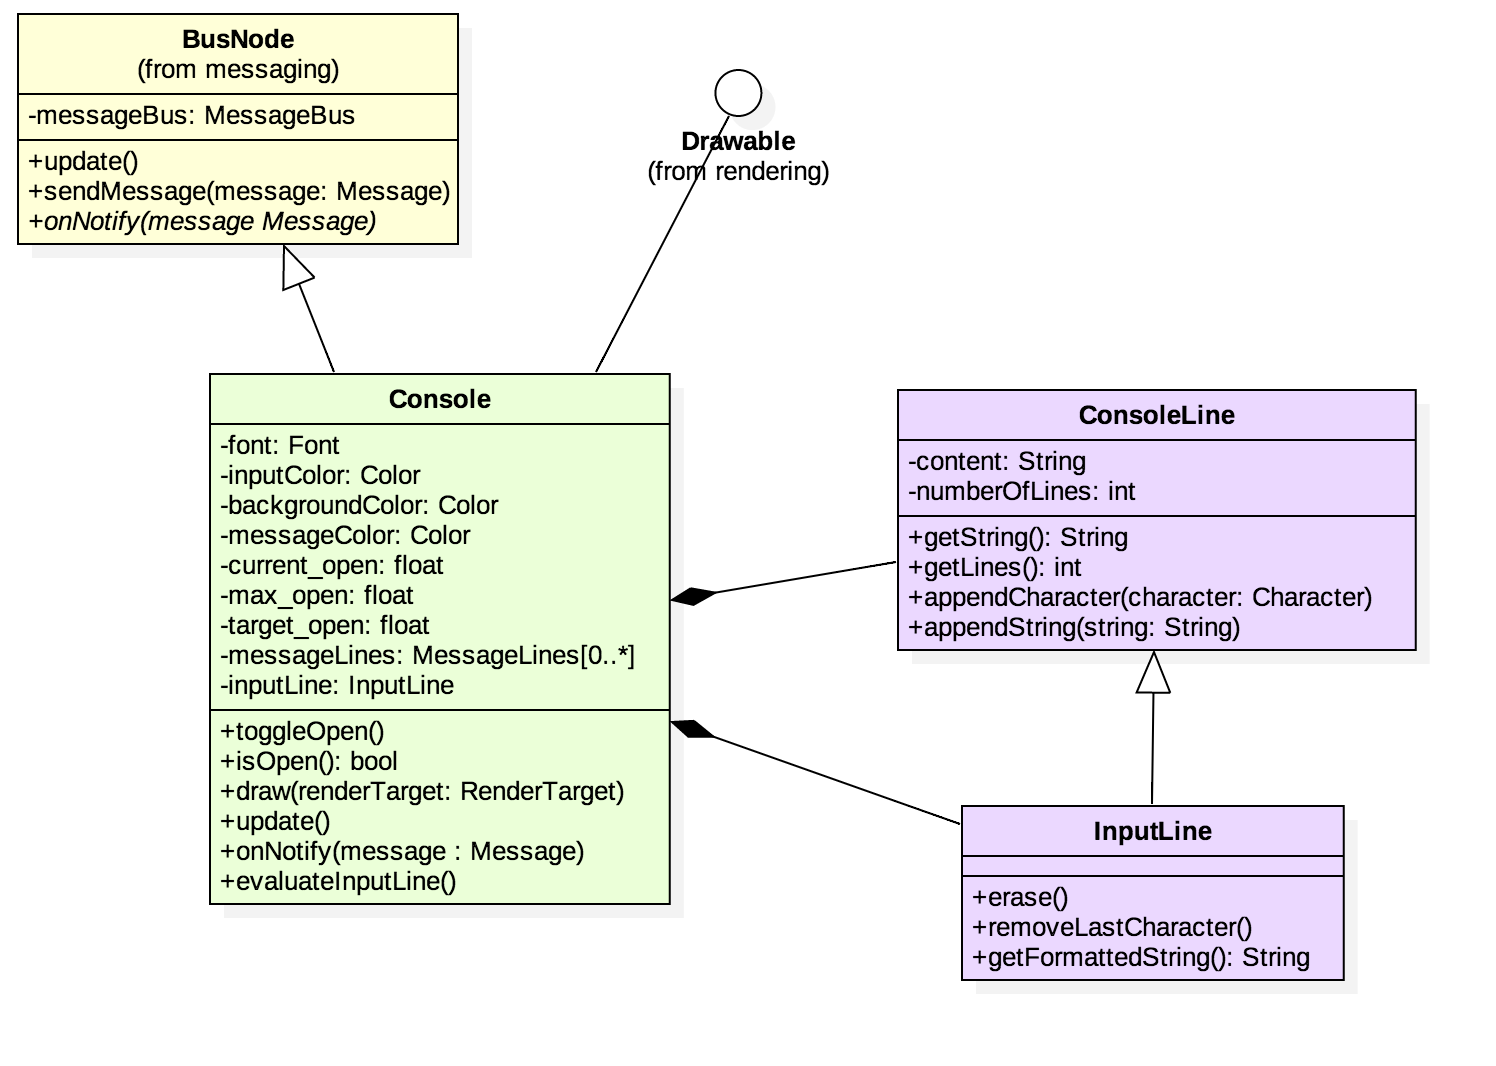
\includegraphics[width=15cm]{otros/UML/png/alld/png/console__diagramaDeClases_console_3.png}}
	\caption{Diagrama de clases del subsistema de consola}
	\label{class:console}
\end{figure}

En la figura \ref{class:console} se ven las clases que componen el subsistema de la consola. En el mismo, la clase \textbf{\textit{Consola}} es la que contiene todas las funcionalidades necesarias, como abrirse y cerrarse con el método \textit{toggleOpen}, ser dibujada con el método \textit{draw} o evaluar la cadena de texto introducida con \textit{evaluateInputLine}.

\bigskip

Vemos además la jerarquía de \textit{ConsoleLine} e \textit{InputLine}. Se encargan respectivamente de contener todas las lineas de texto a mostrar en la consola y de contener el texto introducido por el usuario. \textit{InputLine} extiende a \textit{ConsoleLine} en el sentido de que agrega las funcionalidades necesarias para agregar texto, eliminarlo y ser mostrara con un formato diferente.

\subsubsection*{Subsistema de entrada}

\begin{figure}
	\centerline{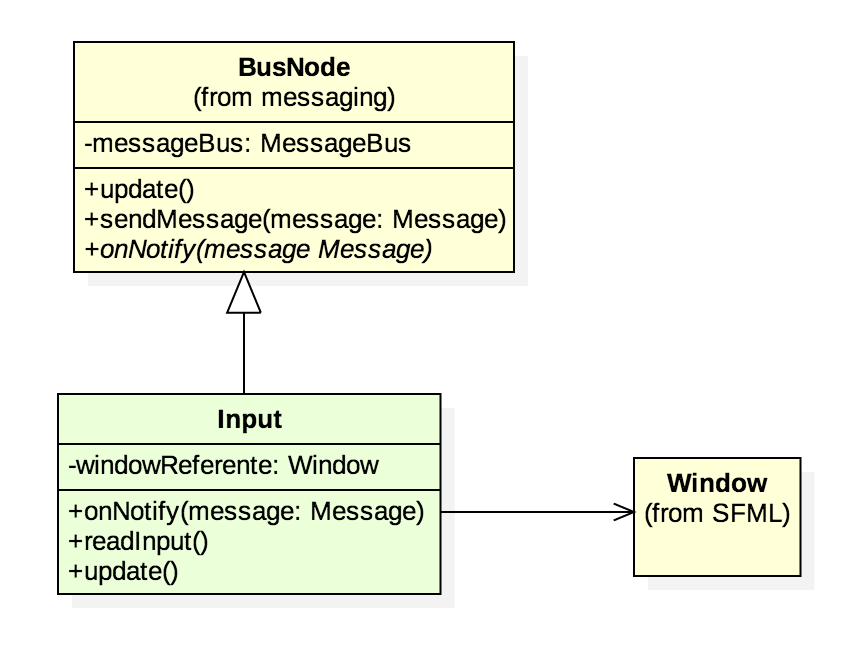
\includegraphics[width=12cm]{otros/UML/png/alld/png/input__diagramaDeClases_input_8.png}}
	\caption{Diagrama de clases del subsistema de entrada}
	\label{class:input}
\end{figure}

La figura \ref{class:input} muestra las clases referentes al subsistema de entrada. En dicho diagrama se puede observar cómo su definición es muy sencilla ya que solamente tendrá que iterar sobre todos los eventos de entrada que ocurren y enviarlos al bus de mensajes.

\bigskip

La clase principal \textit{Input} tendrá una asociación con la clase \textit{Window} de \textit{SFML} ya que es dicha clase la que genera todos los eventos. Internamente, dentro de la función \textit{update}, se irán recogiendo los eventos y enviándolos al bus de mensajes con el mensaje adecuado.


\subsubsection*{Subsistema de físicas}

\begin{figure}
	\centerline{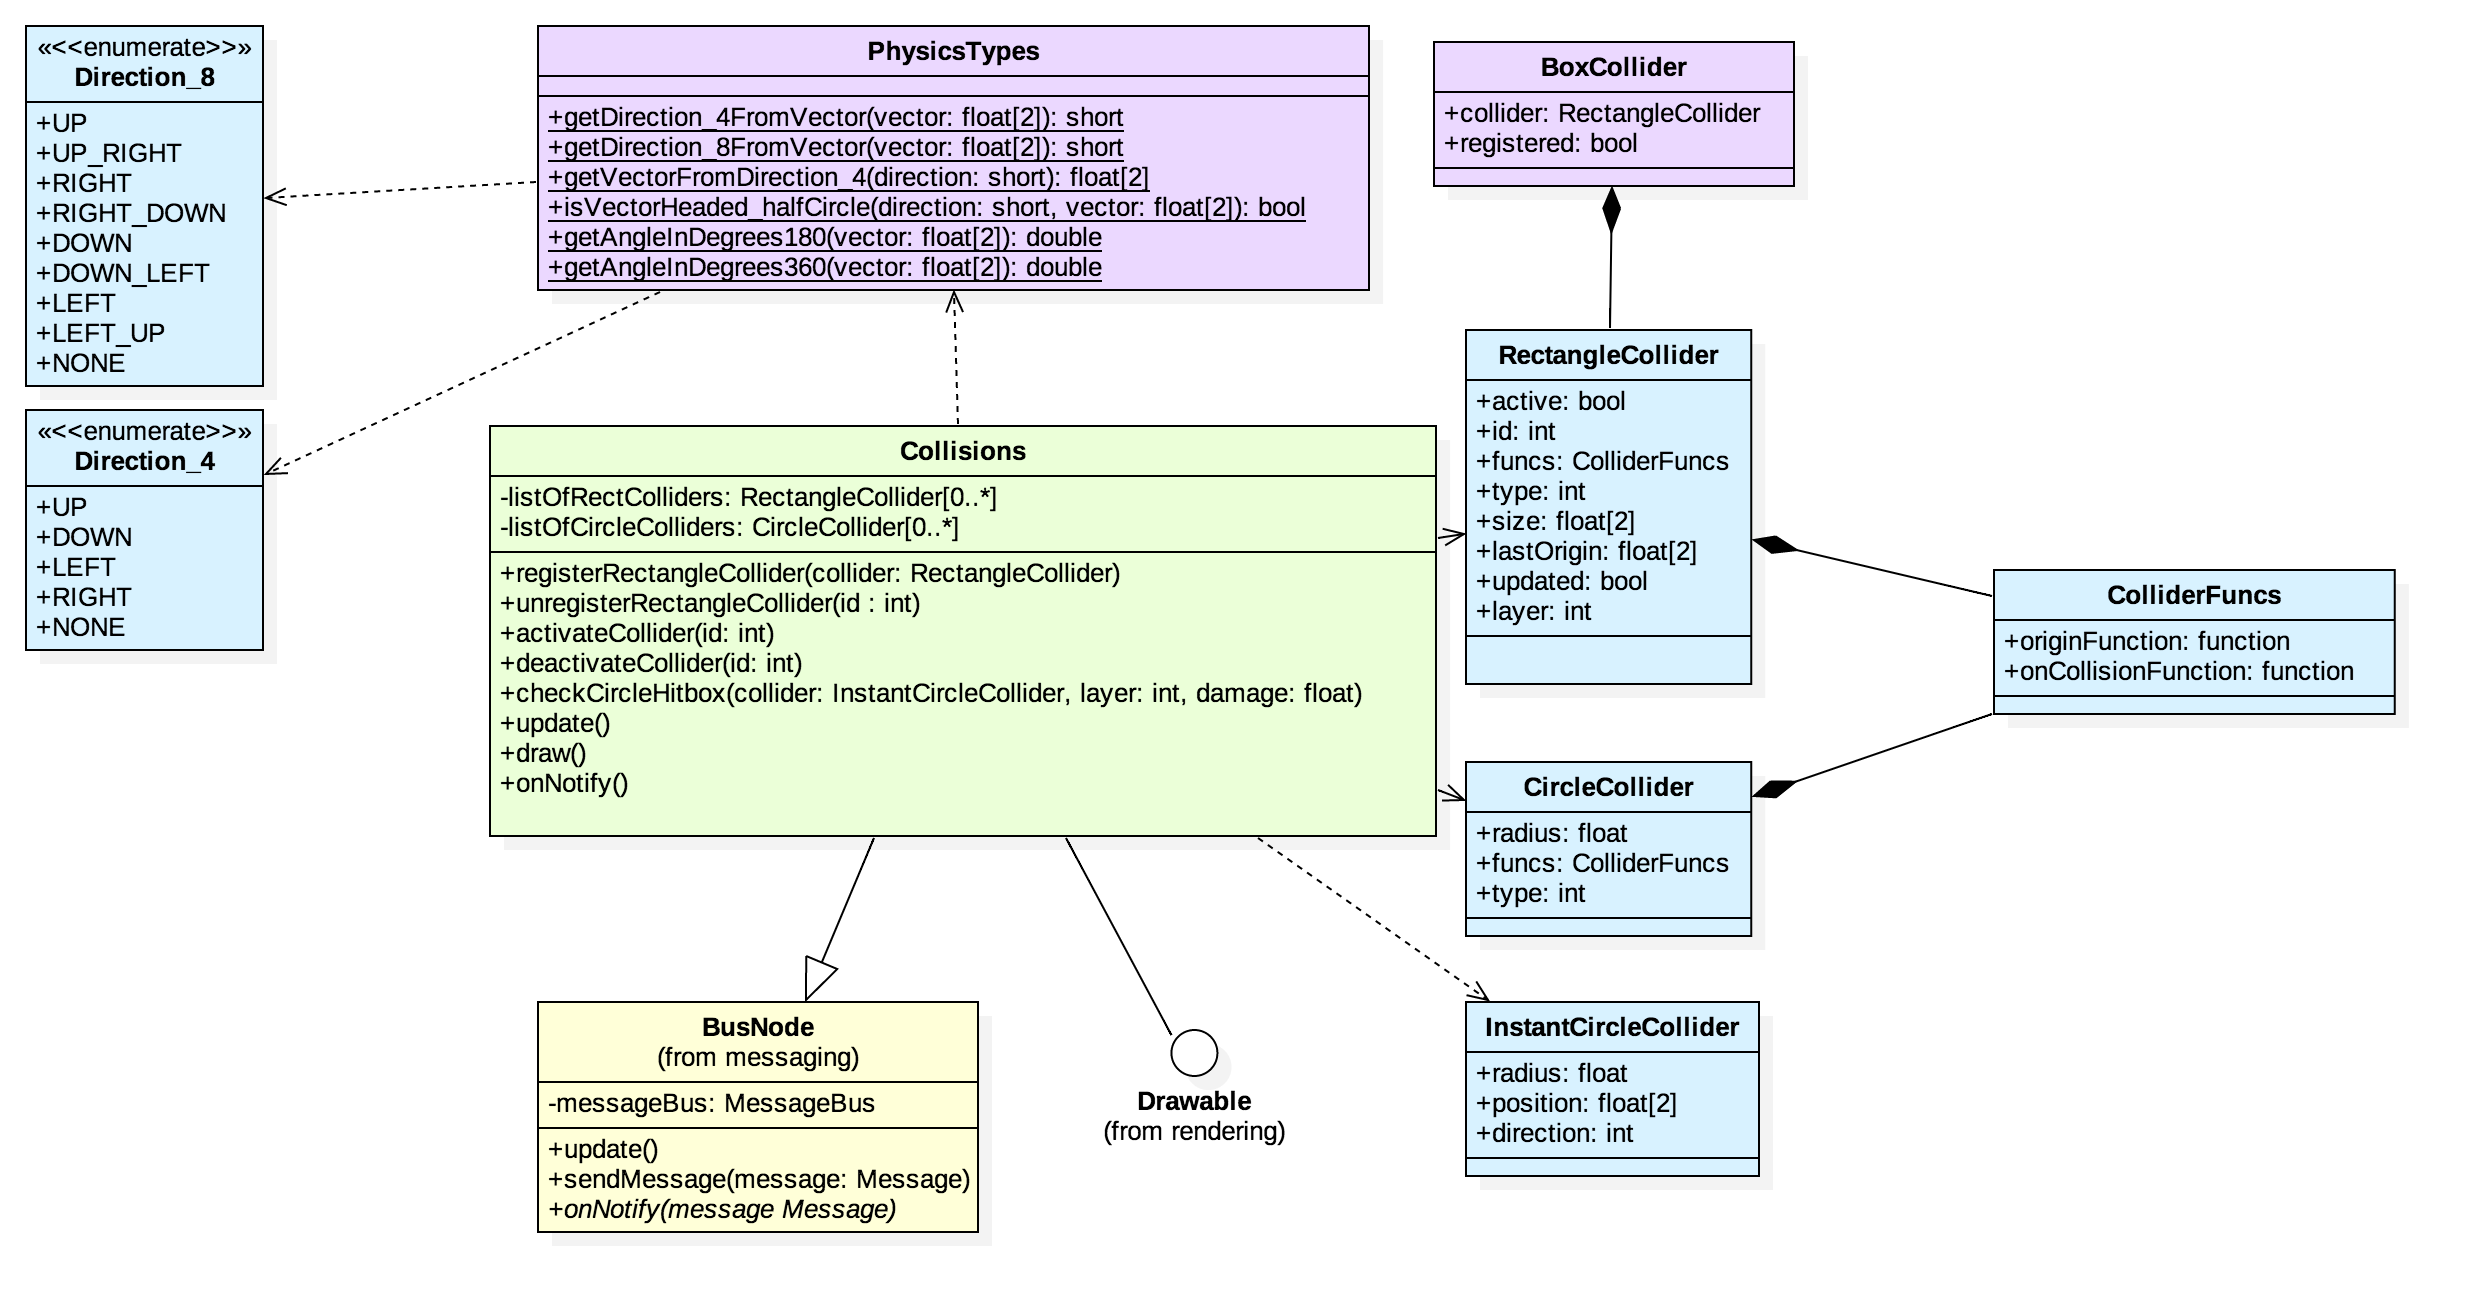
\includegraphics[width=18cm]{otros/UML/png/alld/png/physics__diagramaDeClases_physics_2.png}}
	\caption{Diagrama de clases del subsistema de físicas}
	\label{class:collisions}
\end{figure}

El subsistema de físicas está representado en el diagrama de clases de la figura \ref{class:collisions}. En el mismo destaca la clase \textit{\textbf{Collisions}} que se encarga de guardar los \textit{\textbf{RectangleColliders}} y \textbf{\textit{CircleColliders}} de la aplicación. Estos \textit{colliders} representan las diferentes figuras que pueden sufrir colisiones dentro de una escena y pueden tener forma de rectángulo o círculo. Ambos \textit{colliders} también contienen referencias a funciones capaces de proveer la posición actual del collider y que contienen la función a ejecutar si ocurre una colisión. Dichas funciones las contiene la estructura \textbf{\textit{ColliderFuncs}}.

\bigskip
\textbf{\textit{InstantCircleCollider}} es una estructura que permite comprobar instantáneamente si un circulo arbitrario colisiona con algún otro \textit{collider}. La inmediatez que esto permite es especialmente importante para comprobar si un ataque de un personaje ha acertado o no. Por otra parte, \textbf{\textit{BoxCollider}} es una clase que encapsula un \textit{RectangleCollider} para hacer transparente su creación y registro a otras clases de la aplicación.

\bigskip
Finalmente, \textbf{\textit{PhysicsTypes}} contendrá estructuras que representan direcciones en 4 u 8 sentidos (\textbf{\textit{Direction\_4}} y \textbf{\textit{Direction\_8}} respectivamente) y apostará funciones útiles para trabajar con ellos.


\subsubsection*{Subsistema de renderizado}

\begin{figure}
	\centerline{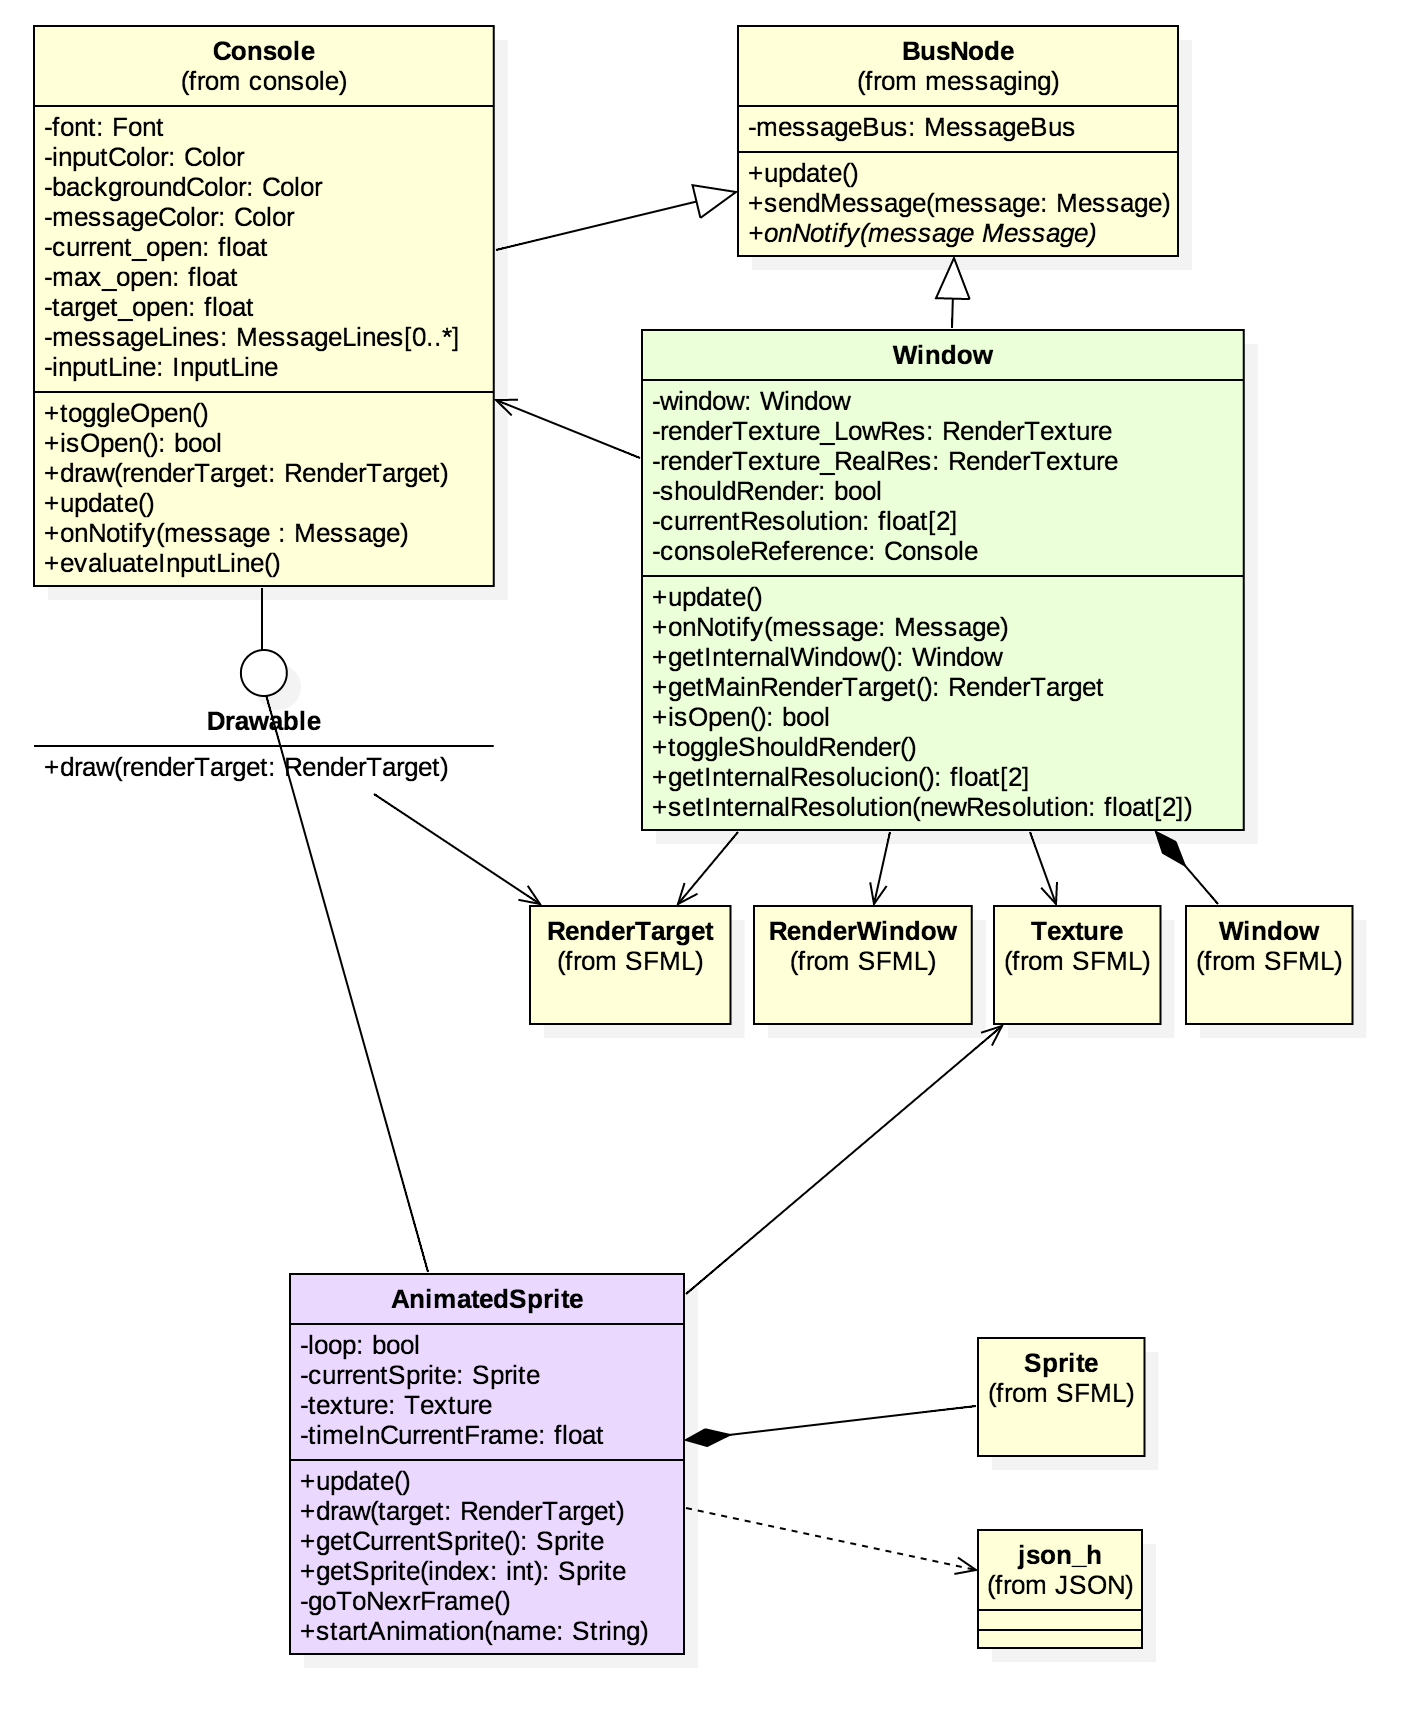
\includegraphics[width=15cm]{otros/UML/png/alld/png/rendering__diagramaDeClases_rendering_9.png}}
	\caption{Diagrama de clases del subsistema de renderizado}
	\label{class:rendering}
\end{figure}

El subsistema de renderizado, mostrado en la figura \ref{class:rendering}, contiene la clase principal \textbf{\textit{Window}} encargada de mostrar por pantalla la aplicación. Para ello aporta funcionalidades como:

\begin{itemize}
	\item Parar de mostrar o volver a mostrar la aplicación con \textit{toggleShouldRender}.
	\item Cambiar la resolución interna de la aplicación independientemente de la externa con \textit{setInternalResolution}.
	\item Comprobar si la ventana sigue abierta para terminar la aplicación.
\end{itemize}

Para dibujar por pantalla hará uso de una serie de atributos, muchos de ellos aportados por la librería \textit{SFML}:

\begin{itemize}
	\item \textbf{\textit{window}}: Objeto de la clase \textit{Window} de \textit{SFML} que representa la funcionalidad más básica de una ventana en el sistema operativo en el que se está ejecutando.
	\item \textbf{\textit{renderTextures}}: Dos objetos de la clase \textit{RenderTexture} de \textit{SFML} que representan texturas sobre las que se dibuja, una de ellas estará a baja resolución y se pintará el juego sobre ella para ahorrar recursos. Luego se escalará esa misma textura y se pintará por encima de la de alta resolución que es la que finalmente se muestra por pantalla.
	\item \textbf{\textit{shouldRender}}: Booleano que define si se muestra o no algo por pantalla.
	\item \textbf{\textit{currentResolution}}: Que guarda la resolución real de la ventana.
	\item \textbf{\textit{consoleReferente}}: Referencia a la consola que permite pintarla siempre que sea necesario, independientemente de que exista una escena o de que el juego se encuentre detenido.
\end{itemize}

\bigskip

Además, la clase \textbf{\textit{AnimatedSprite}} guarda una textura en formato png que contiene todos los dibujos de un personaje en las diferentes posturas que forma una animación, lo que se conoce como \textit{spritesheet}. Para mostrar el dibujo correcto se lee previamente un archivo en formato JSON con ayuda de \textbf{\textit{json.h}} que contiene las animaciones y donde están localizadas cada imagen individual dentro de la textura general.

\bigskip

Esta clase ofrece una forma general de guardar y mostrar movimiento de cara a \textit{gameobjects} con animaciones.

\subsubsection*{Subsistema de renderizado}

\begin{figure}
	\centerline{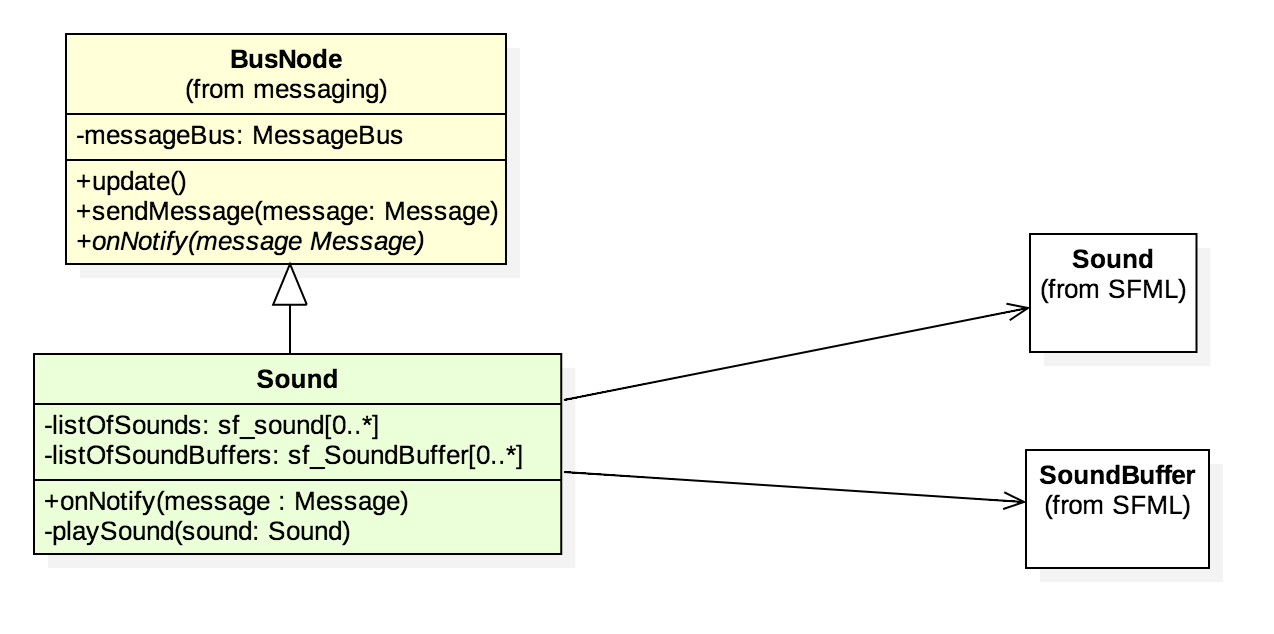
\includegraphics[width=15cm]{otros/UML/png/alld/png/sound__diagramaDeClases_sound_1.png}}
	\caption{Diagrama de clases del subsistema de sonido}
	\label{class:sound}
\end{figure}

Finalmente, se puede observar el diagrama del subsistema de sonido en la figura \ref{class:sound}. El mismo es muy sencillo, ya que los sonidos (representados por la clase \textbf{\textit{Sound}}) unicamente son cargados al inicializar el subsistema, junto con los \textit{buffers} (representados por la clase \textbf{\textit{SoundBuffer}}) necesarios para su reproducción que guardan datos referentes a cada \textit{tick} dentro del archivo de sonido.

\bigskip

Internamente, se utilizarán dos listas con dichos sonidos y \textit{buffers} que serán accedidos cuando se utilice la función \textbf{\textit{playSound}} para comenzar la reproducción de un sonido. La única forma de que se ejecute \textit{playSound} es que llegue un mensaje concreto para cada sonido desde el bus de mensajes.

\subsection{Otros útiles}

\subsubsection*{Paquete de recursos}

\begin{figure}
	\centerline{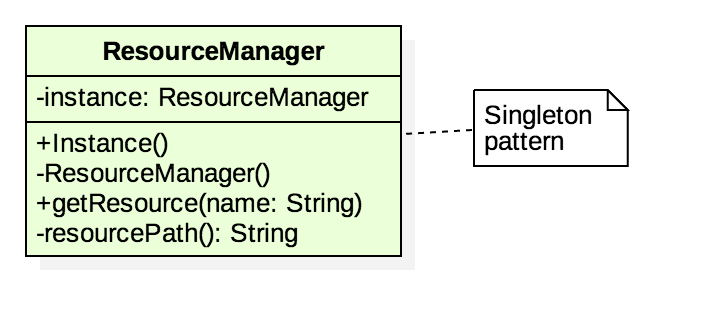
\includegraphics[width=8cm]{otros/UML/png/alld/png/resources__diagramaDeClases_resources_0.png}}
	\caption{Diagrama de clases del paquete de recursos}
	\label{class:resources}
\end{figure}

La clase \textbf{\textit{ResourceManager}} mostrada en la figura \ref{class:resources} es la encargada de hacer que todos los recursos que necesita el juego estén disponibles en tiempo de ejecución. Para lograr esto se ha implementado un \textit{Singleton} que contiene partes en el lenguaje \textit{Objective-C}. Esto permite trabajar directamente con el sistema operativo de Apple y acceder a recursos embebidos dentro del ejecutable \textit{.app} de la aplicación.

\bigskip

La funcionalidad básica de \textbf{\textit{getResource}} buscará y devolverá un recurso determinado con el nombre dado. Además, la función de \textbf{\textit{resourcePath()}} devolverá siempre una ruta válida hasta los recursos de la aplicación (fuentes, sonidos, imágenes, etc.).

\subsubsection*{Paquete de útiles}

\begin{figure}
	\centerline{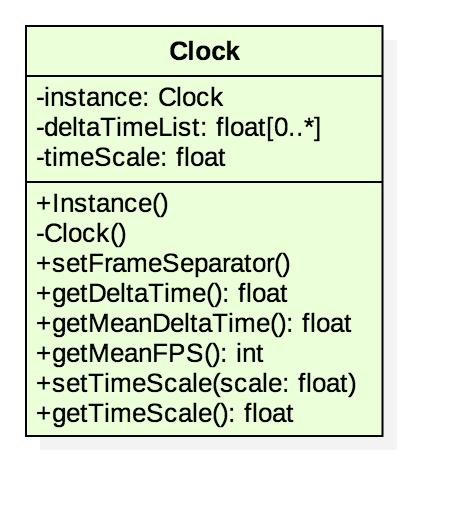
\includegraphics[width=5cm]{otros/UML/png/alld/png/utils__diagramaDeClases_utils_10.png}}
	\caption{Diagrama de clases del paquete de útiles}
	\label{class:utils}
\end{figure}

Por último se muestra el paquete de utilidades comunes en la figura \ref{class:utils}. El mismo solo contiene la clase \textbf{\textit{Clock}}, un \textit{Singleton} que representa el reloj interno de la aplicación. El mismo es capaz de determinar el tiempo que ha transcurrido entre fotogramas para calcular de forma precisa el movimiento y físicas del videojuego.

\bigskip

Además proporciona la posibilidad de escalar su velocidad mediante \textbf{\textit{setTimeScale}} permitiendo así las simulaciones aceleradas referenciadas en el RNF-2.

\bigskip

Este paquete podría contener cualquier funcionalidad común y útil para varios subsistemas pero ya que las mismas están convenientemente encapsuladas en dicho subsistemas no ha sido necesario agrupar muchas funcionalidades en el presente paquete.

\subsection{Escenas}

\subsubsection*{Escena del menú}

\begin{figure}
	\centerline{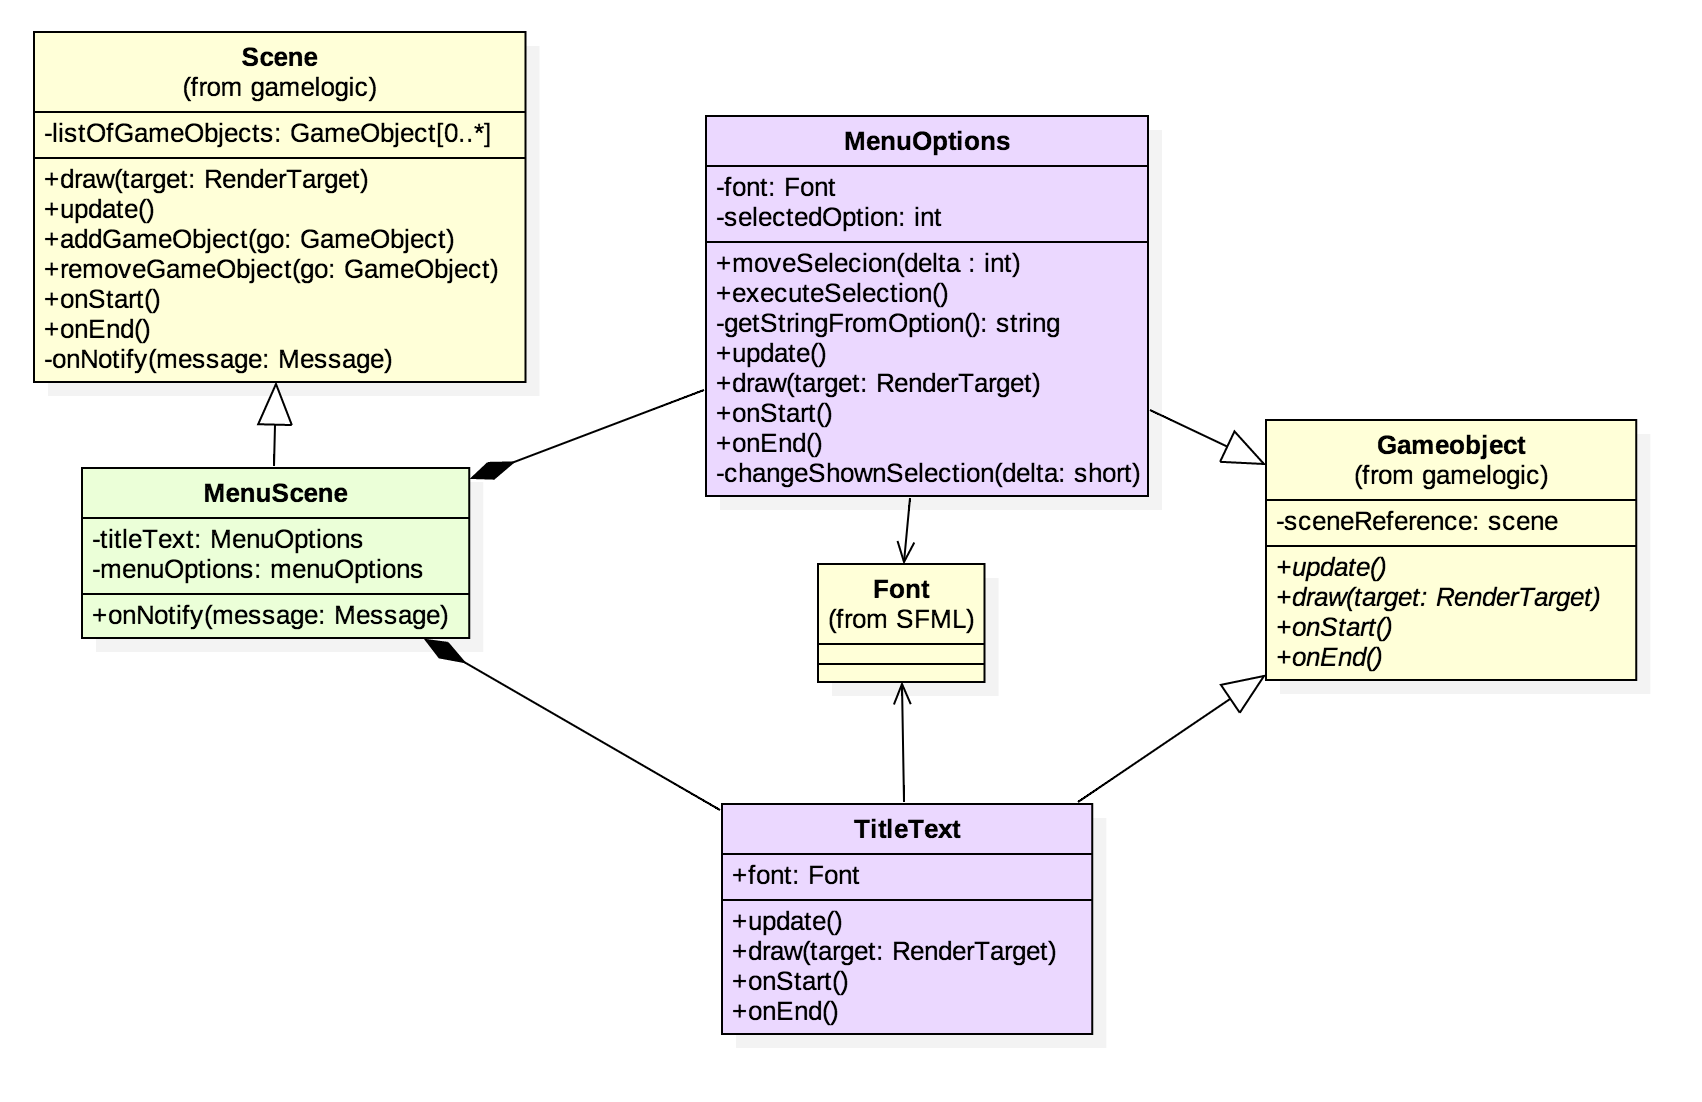
\includegraphics[width=15cm]{otros/UML/png/alld/png/gamelogic__menu__diagramaDeClases_scene_menu_6.png}}
	\caption{Diagrama de clases de la escena del menú}
	\label{class:menu}
\end{figure}

La escena del menú, mostrada en la figura \ref{class:menu}, es la escena más sencilla de la aplicación. Contiene los siguientes \textit{gameobjects}:

\begin{itemize}
	\item \textbf{\textit{TitleText}}: Simplemente usado para mostrar el título del juego.
	\item \textbf{\textit{MenuOptions}}: Contiene las diferentes opciones del menú, se encarga de guardar la que está seleccionada, cambiar esta selección y ejecutar la seleccionada cuando se requiere.
\end{itemize}

\subsubsection*{Escena de juego}

\begin{figure}
	\caption{Diagrama de clases de la escena de juego}
	\hspace*{-0.1cm}  
	\centerline{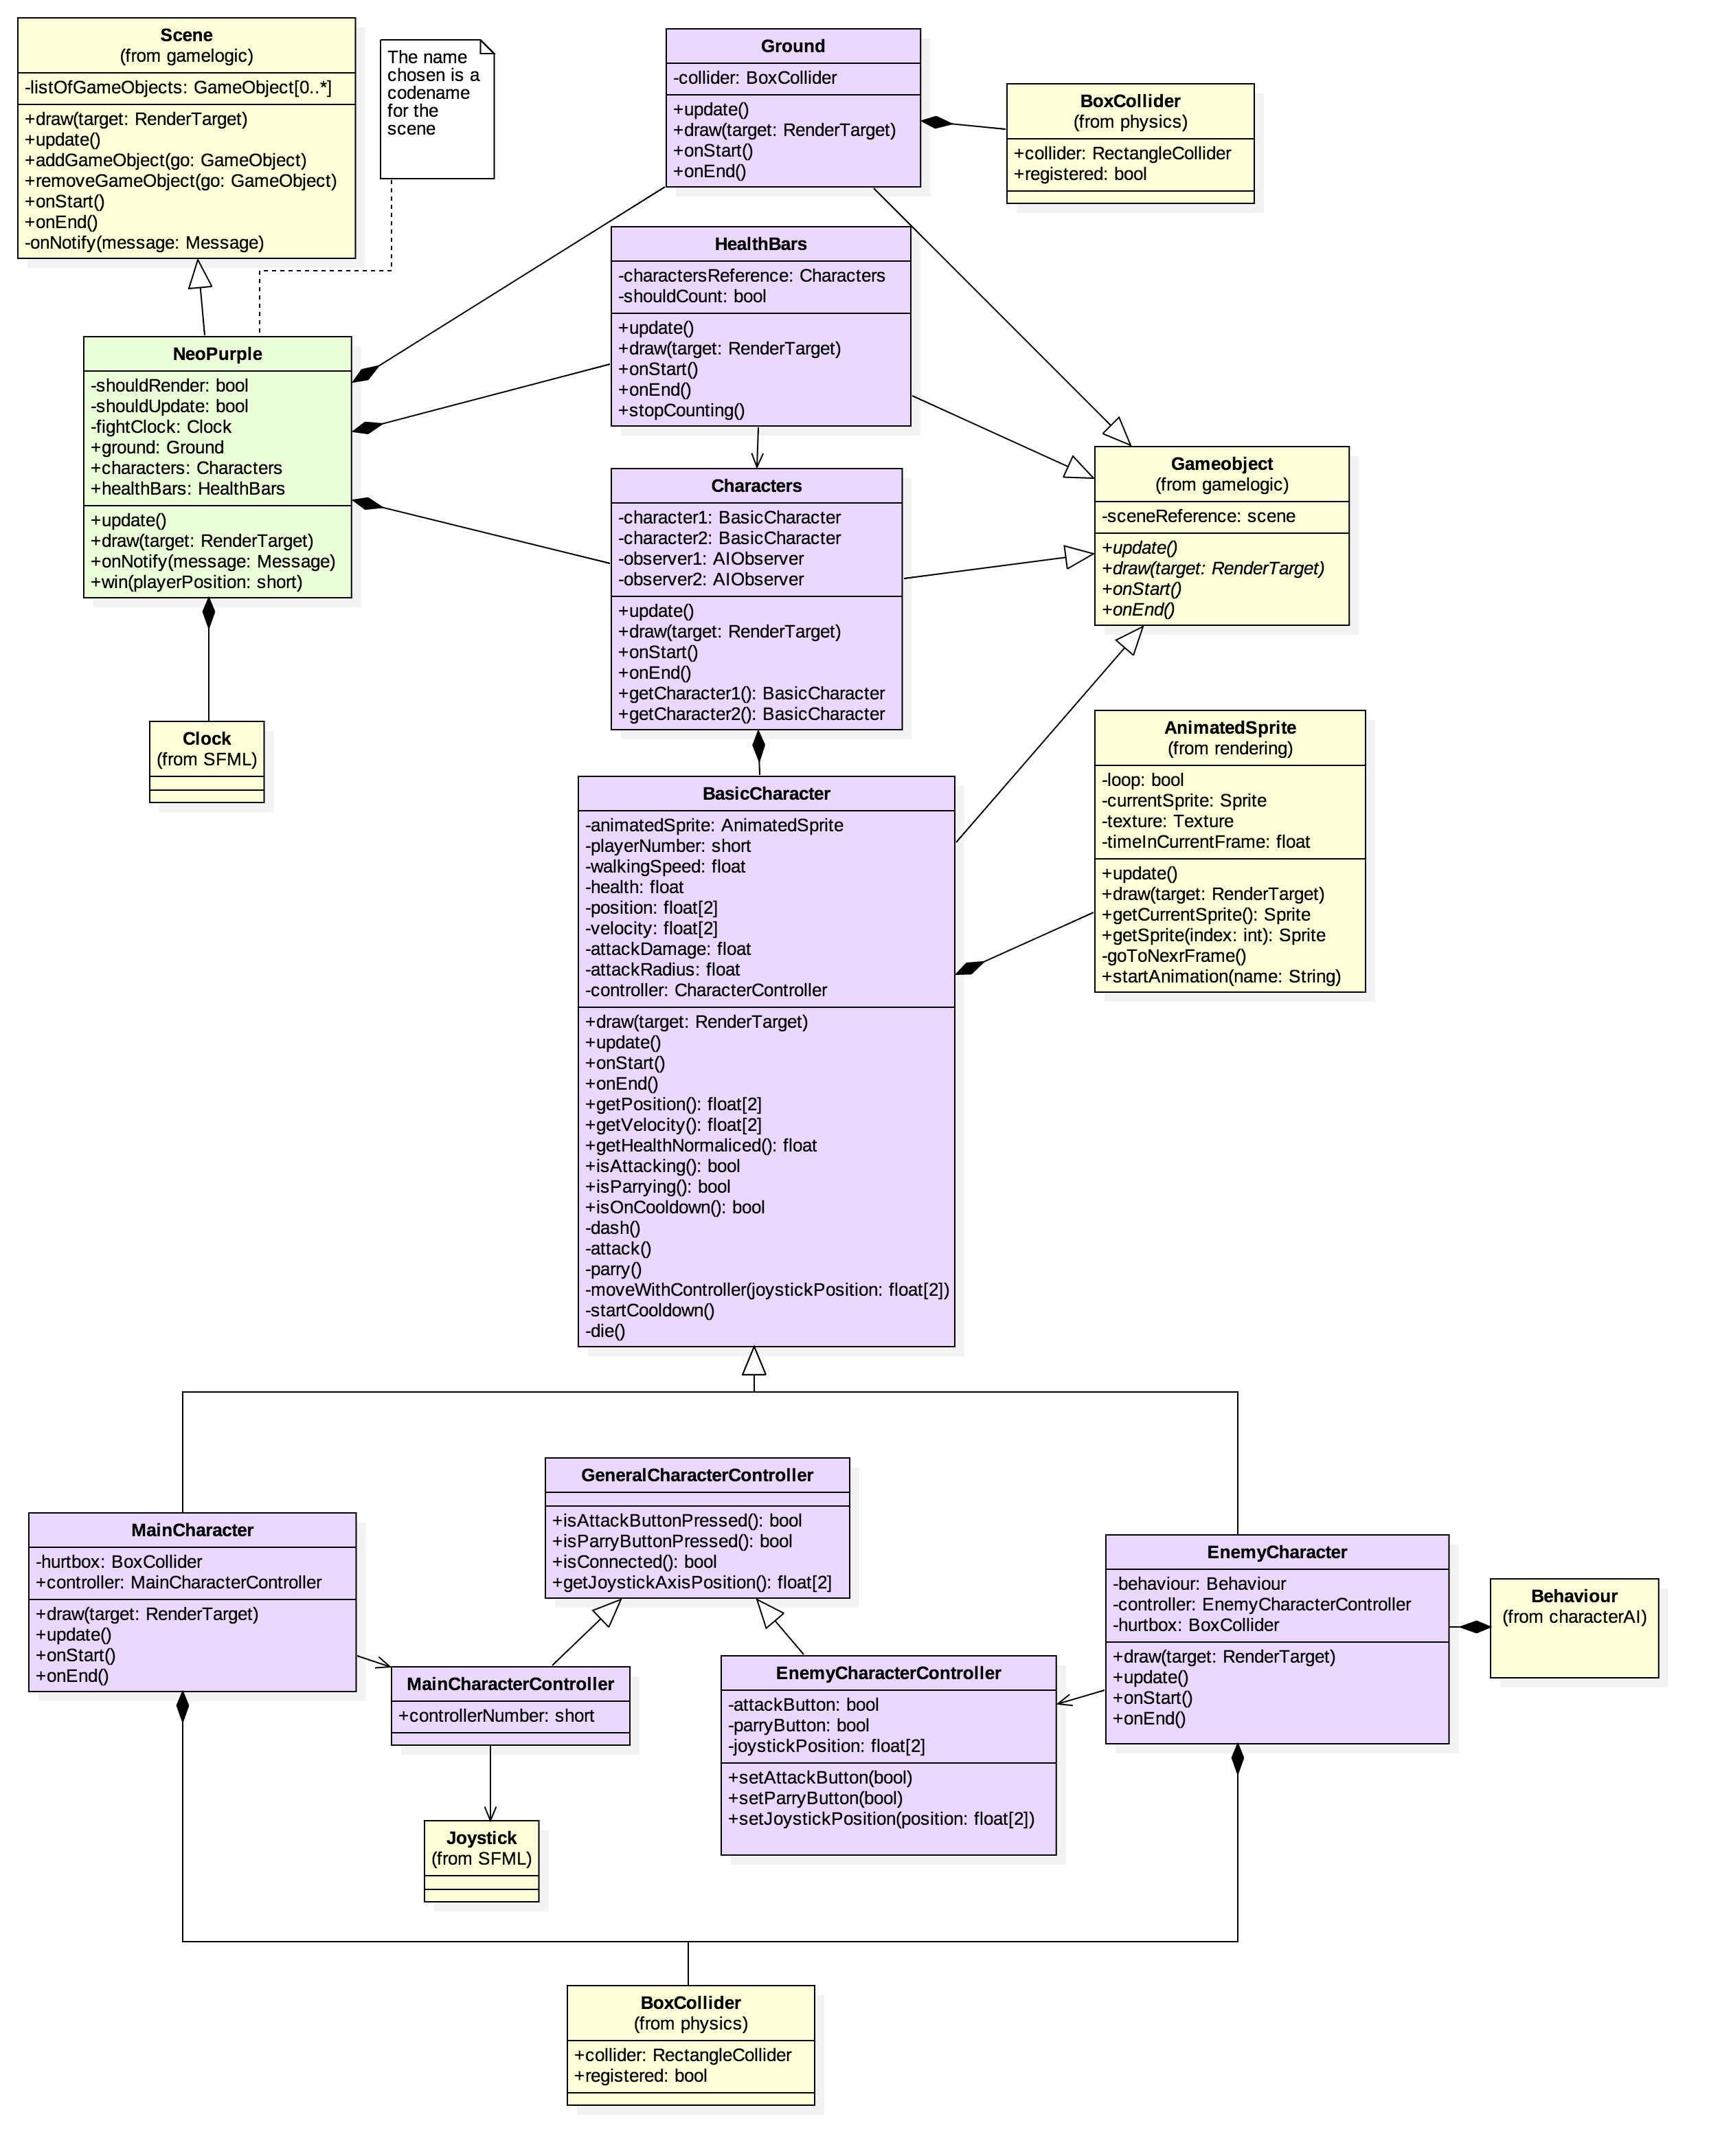
\includegraphics[width=20cm]{otros/UML/png/alld/png/gamelogic__gameplay__diagramaDeClases_scene_gameplay_4.png}}
	\label{class:gameplay}
\end{figure}

Esta escena (figura \ref{class:gameplay}) es la dedicada a jugar realmente al videojuego, la misma contiene el combate entre los dos personajes. La clase dedicada a la escena es \textbf{\textit{NeoPurple}}\footnote{Nombre en clave escogido por la apariencia del suelo de la escena para identificarla fácilmente en caso de que se requirieran más escenas con \textit{gameplay}} y se encarga de contener a todos los \textit{gameobjects} necesarios y a gestionar la victoria de uno de los personajes con la función \textbf{\textit{win}}. Los \textit{gameobjects} contenidos en la escena son:

\begin{itemize}
	\item \textbf{\textit{Ground}}: Encargado de representar el suelo de la escena, es el encargado tanto de pintar el suelo como de proporcionar al sistema de colisiones un \textit{collider} que impida que los personajes se salgan de la escena mediante el uso de ese \textit{BoxCollider}.
	\item \textbf{\textit{HealthBars}}: Muestra la vida de los dos personajes y el tiempo de pelea restante, tiene una referencia a \textit{Characters} para obtener información sobre la vida de ambos.
	\item \textbf{\textit{Characters}}: Contiene e identifica a los dos personajes en la escena, no solo facilita acceder a ellos por parte de las clases que lo requieran sino que ayuda a reconocer cual es el personaje 1 y 2 y saber por que están siendo controlados (jugador, agente, sistema de reglas, etc).
	\item \textbf{\textit{BasicCharacter}}: Clase genérica que representa un personaje, contiene todas las funciones de movimiento y acciones que el mismo puede realizar (\textit{attack}, \textit{parry} y \textit{moveWithController}). Además contiene todos los atributos que definen sus características como la vida (\textit{health}), rango (\textit{attackRadius}), velocidad (\textit{velocity}), posición (\textit{position}), daño (\textit{attackDamage}), etc. 
	\item \textbf{\textit{MainCharacter}}: Clase que representa a un personaje controlado por el jugador, hace uso de la clase \textbf{\textit{MainController}} que representa un mando real conectado el equipo.
	\item \textbf{\textit{EnemyCharacter}}: Clase que representa a un personaje controlado por la aplicación, contiene un mando virtual representado por \textbf{\textit{EnemyController}} que será modificado por el comportamiento o \textbf{\textit{Behaviour}} del que se habla en el siguiente apartado.
\end{itemize}

\bigskip

Ambos personajes cuentan con una instancia de \textit{BoxCollider} que representa el \textit{collider} usado para recibir daño.

\subsubsection*{Comportamiento del agente}
\label{cap:diseno:agente}
El diagrama contenido en la figura \ref{class:agent} es uno de los más complejos de la aplicación. De hecho, debería de estar en la figura \ref{class:gameplay} ya que forma parte del \textit{gameplay} pero dada su importancia y complejidad se ha decidido dedicar esta sección al mismo en aras de evitar diagramas enormes imposibles de ver en un documento de este formato y de entender a primera vista. Para explicar sus partes se dedicará una parte deparada a cada uno de los conjuntos de componentes.

\bigskip

Comenzando por la parte izquierda se ven las clases que representan el estado de la pelea a ojos del agente. La versión continua del estado está contenida en \textbf{\textit{FightState}} que contendrá el estado de ambos personajes representado por la clase \textbf{\textit{CharacterState}}.

\bigskip
La clase \textbf{\textit{Observer}} es el componente encargado de representar los \textit{ojos} del agente en el sentido de ver la situación de los personajes y representarla de un modo adecuado. Por lo tanto, será este el encargado de discretizar el estado continuo para obtener un objeto de la clase \textbf{\textit{FightState\_Discrete}}. Esta clase contiene el estado propio del personaje y del enemigo en \textbf{\textit{MyCharacterState\_Discrete}} y \textbf{\textit{OtherCharacterState\_Discrete}} respectivamente. Es importante mencionar que solo el estado propio contiene datos de posición ya que la misma se define de forma relativa al enemigo en la clase \textbf{\textit{Position\_Discrete}} de forma que se evita duplicar información.

\bigskip

Pasando ahora a la jerarquía de clases de \textbf{\textit{Behaviour}} se ve cómo la clase principal es la encargada de representar la estrategia genérica del patrón \textit{Strategy}\ref{pat:strategy} ya que el enemigo siempre tendrá una pero podrá cambiar entre ellas en diferentes ejecuciones. Esta clase \textit{Behaviour} tiene acceso a la clase \textbf{\textit{Actions}} que encapsula las acciones posibles a realizar y las ejecuta con \textbf{\textit{execute}} sobre la referencia al \textit{controller} que contiene. Algo importante es el hecho de que \textit{Behaviour} contiene un \textit{thread} independiente que correrá todos los cálculos referentes a la inteligencia artificial del juego, separando de forma efectiva la complejidad del juego con la del agente y favoreciendo el rendimiento.

\bigskip

\textbf{\textit{RuleBasedBehaviour}} es la implementación base sobre la que probar al agente. La misma especifica las acciones que llevará a cabo el enemigo en cada situación y se ha realizado gracias al \textbf{conocimiento experto} del desarrollador pues el mismo tiene experiencia jugando al juego. Solo necesita acceso al estado actual de la pelea (\textbf{\textit{currentState}}) para elegir la acción programada.

\bigskip

\textbf{\textit{ReinforcementBehaviour}} es la clase que contiene el comportamiento que el agente ha aprendido. El mismo se ha generado a partir de la exploración de estados posibles y de la mejora en la función de \textit{fitness} que ha supuesto cada acción. Para calcular este \textit{fitness} se hace uso de la función \textbf{\textit{calculateFitness}} en \textit{Observer}.

\bigskip

Para representar la información referente a los estados visitados se guarda el estado actual (\textbf{\textit{currentState}}) y el último (\textbf{\textit{lastState}}), además de la ultima acción escogida (\textbf{\textit{lastAction}}). Con estos datos, al principio de cada iteración del \textbf{\textit{update}}, se guardará en el \textit{StateActionContainer} la mejora en el \textit{fitness} asociada a una acción para un determinado estado. Luego se obtendrá el estado actual y si este no ha sido visitado se escogerá una acción aleatoria, si por el contrario este ha sido visitado, se escogerá entre las posibles acciones teniendo en cuenta el \textit{fitness} esperado para cada una, habiendo una posibilidad de que aleatoriamente se escoja una acción con poco \textit{fitness} para solucionar el conocido problema de exploración contra explotación\footnote{Problema común en entornos de inteligencia artificial en el cual un agente debe balancear escoger siempre la opción que parece la mejor en este momento con explorar las otras posibles opciones en busca de otra que pueda ser superior.} en inteligencia artificial.

\bigskip

Por último, \textbf{\textit{StateActionContainer}} será un \textit{Singleton} encargado de representar el conocimiento sobre los estados. Las estructuras que representan este conocimiento son \textbf{\textit{StateActionSituation}} y \textbf{\textit{ActionSituation}} que contienen la información para un estado y para cada acción dentro del estado respectivamente. Además, \textit{StateActionContainer} es capaz de leer y guardar este conocimiento desde un archivo dentro del ejecutable para mantenerlo entre diferentes ejecuciones. Se podría usar la opción de \textbf{\textit{resetKnowledge}} si se quisiera que el agente olvidara todo lo aprendido hasta el momento.


\clearpage
\begin{landscape}
\begin{figure}
	\begin{adjustwidth}{-3cm}{}
		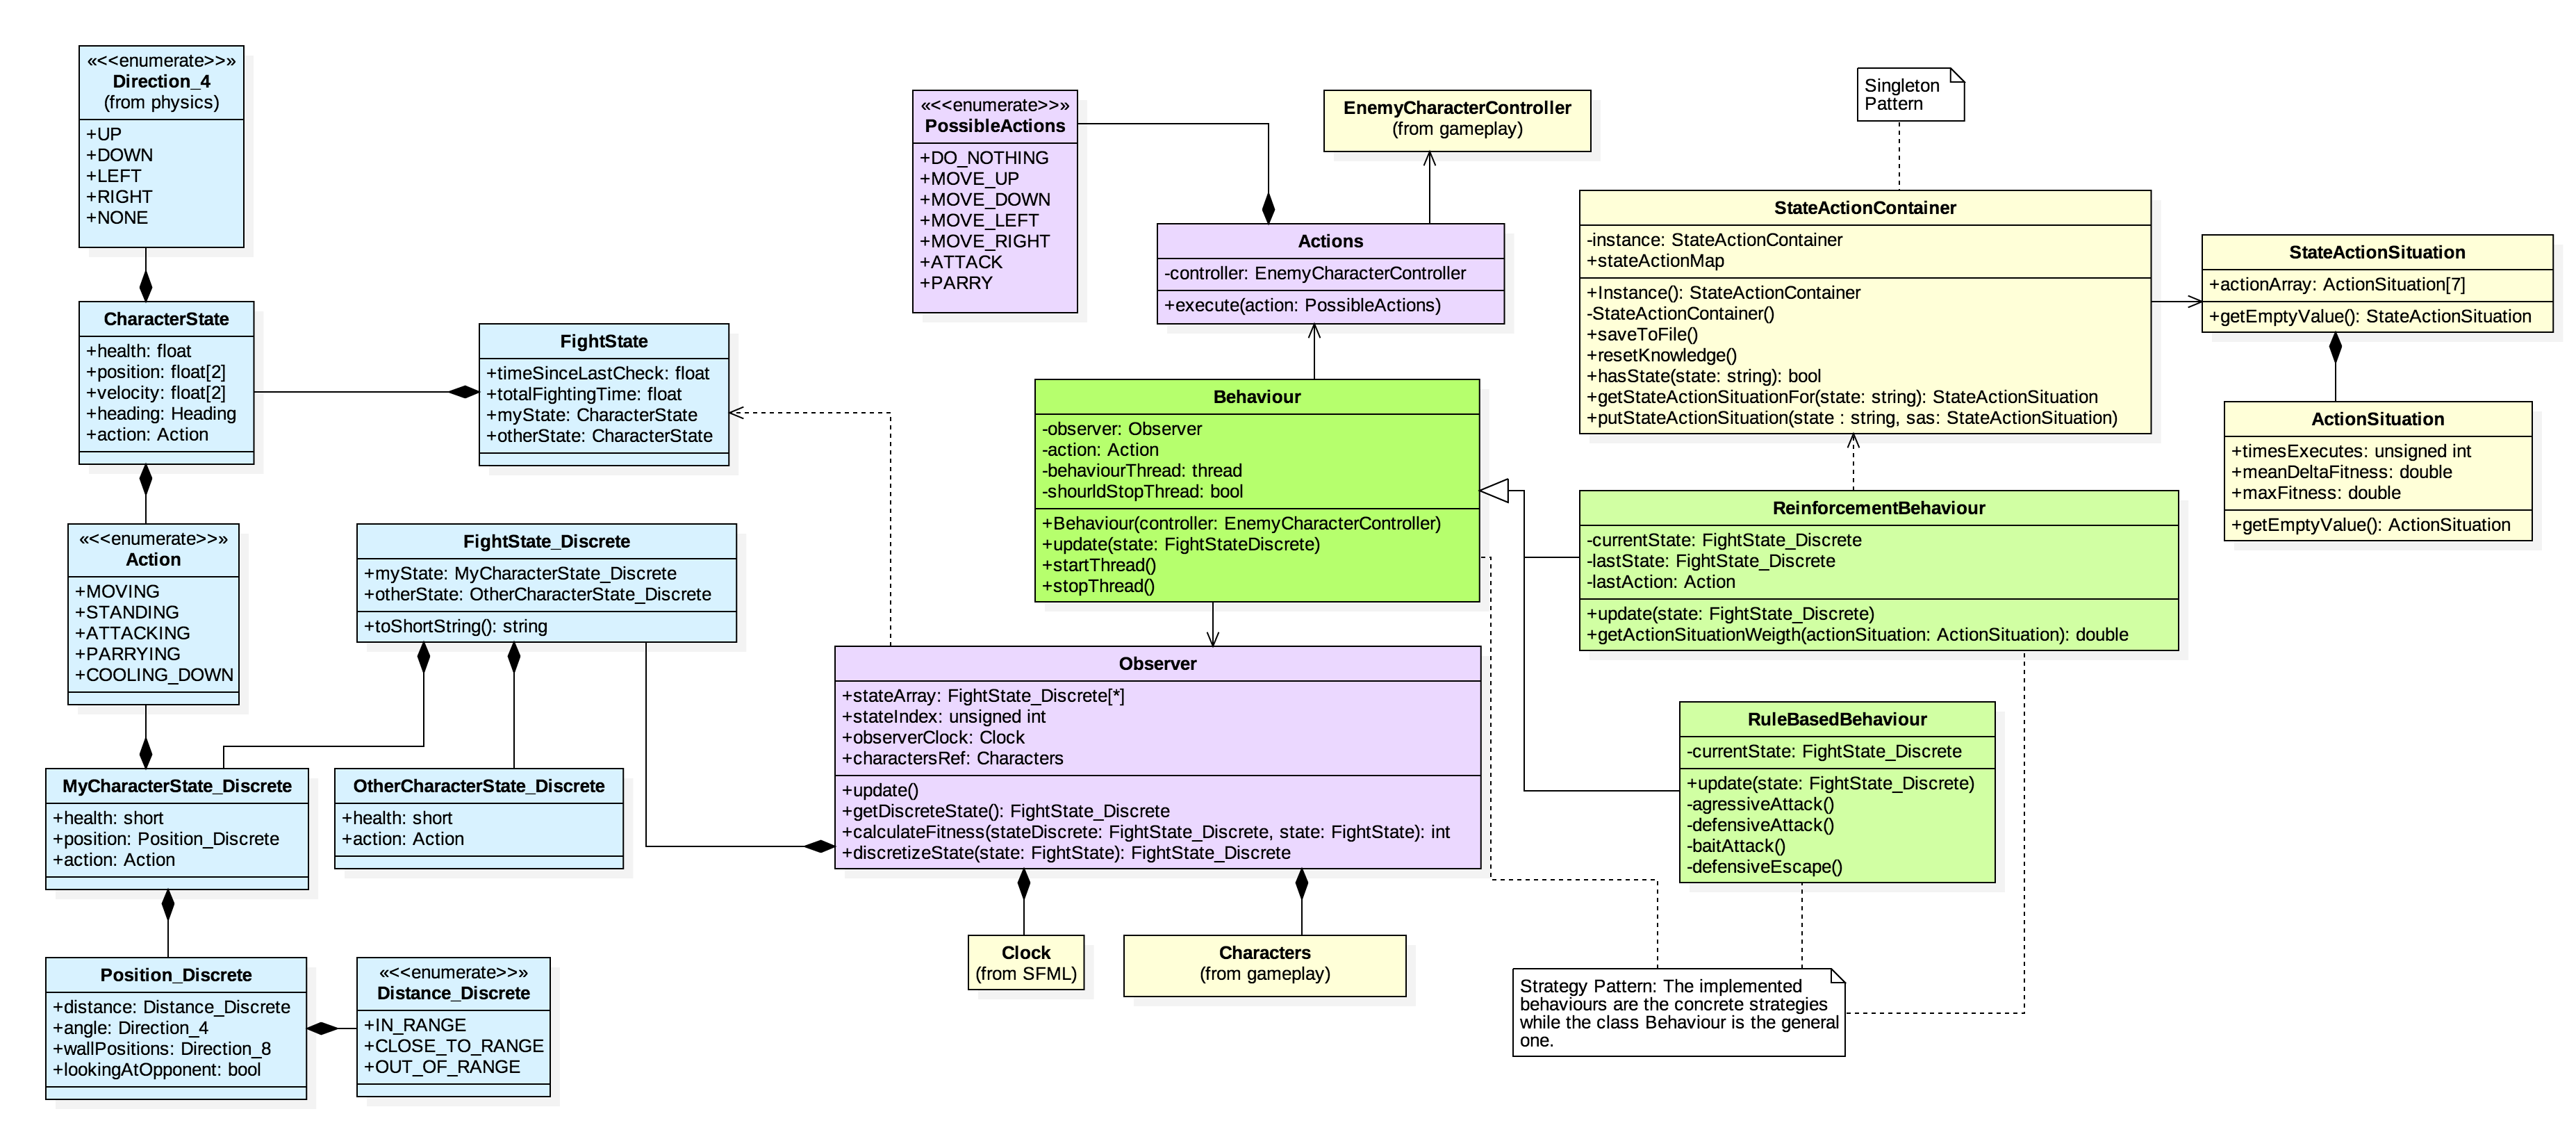
\includegraphics[width=24cm]{otros/UML/png/alld/png/gamelogic__gameplay__characterAI__diagramaDeClases_IA_5.png}
		\caption{Diagrama de clases del comportamiento del agente}
		\label{class:agent}
	\end{adjustwidth}
\end{figure}
\end{landscape}
\clearpage



\section{Diagramas de secuencia}

Esta sección estará dedicada a explicar la secuencia de operaciones que se realiza en casos comunes e importantes de partes de la aplicación. Se ha optado por mostrar partes clave de la aplicación en lugar de dedicar un diagrama de secuencia a cada caso de uso ya que si se hiciera de este modo se repetiría mucha información entre los mismos, además de dar lugar a diagramas de secuencia de tamaños excesivos. Otra nota importante es que no se suelen utilizar diagramas de secuencia en este tipo de arquitecturas y en especial en videojuegos ya que su naturaleza lleva a realizar acciones durante muchas diferentes del \textit{gameloop}\footnote{Bucle principal de un videojuego en el que se actualizan todas sus partes, se puede ver un ejemplo en la figura \ref{sec:general}} haciendo que representar un caso de uso diera lugar a diagramas de secuencia con decenas de instancias y cientos de mensajes entre ellas.

\bigskip

En los siguientes párrafos se mostrarán diagramas de secuencia relevantes de la aplicación y se relacionarán con los casos de uso en los que son importantes. Se empieza por los diagramas asociados a la aplicación en general para luego seguir con los diagramas específicos relacionados con las escenas y el agente.

\subsection{Aplicación general}

\subsubsection*{Aplicación global}

\begin{figure}
	\centerline{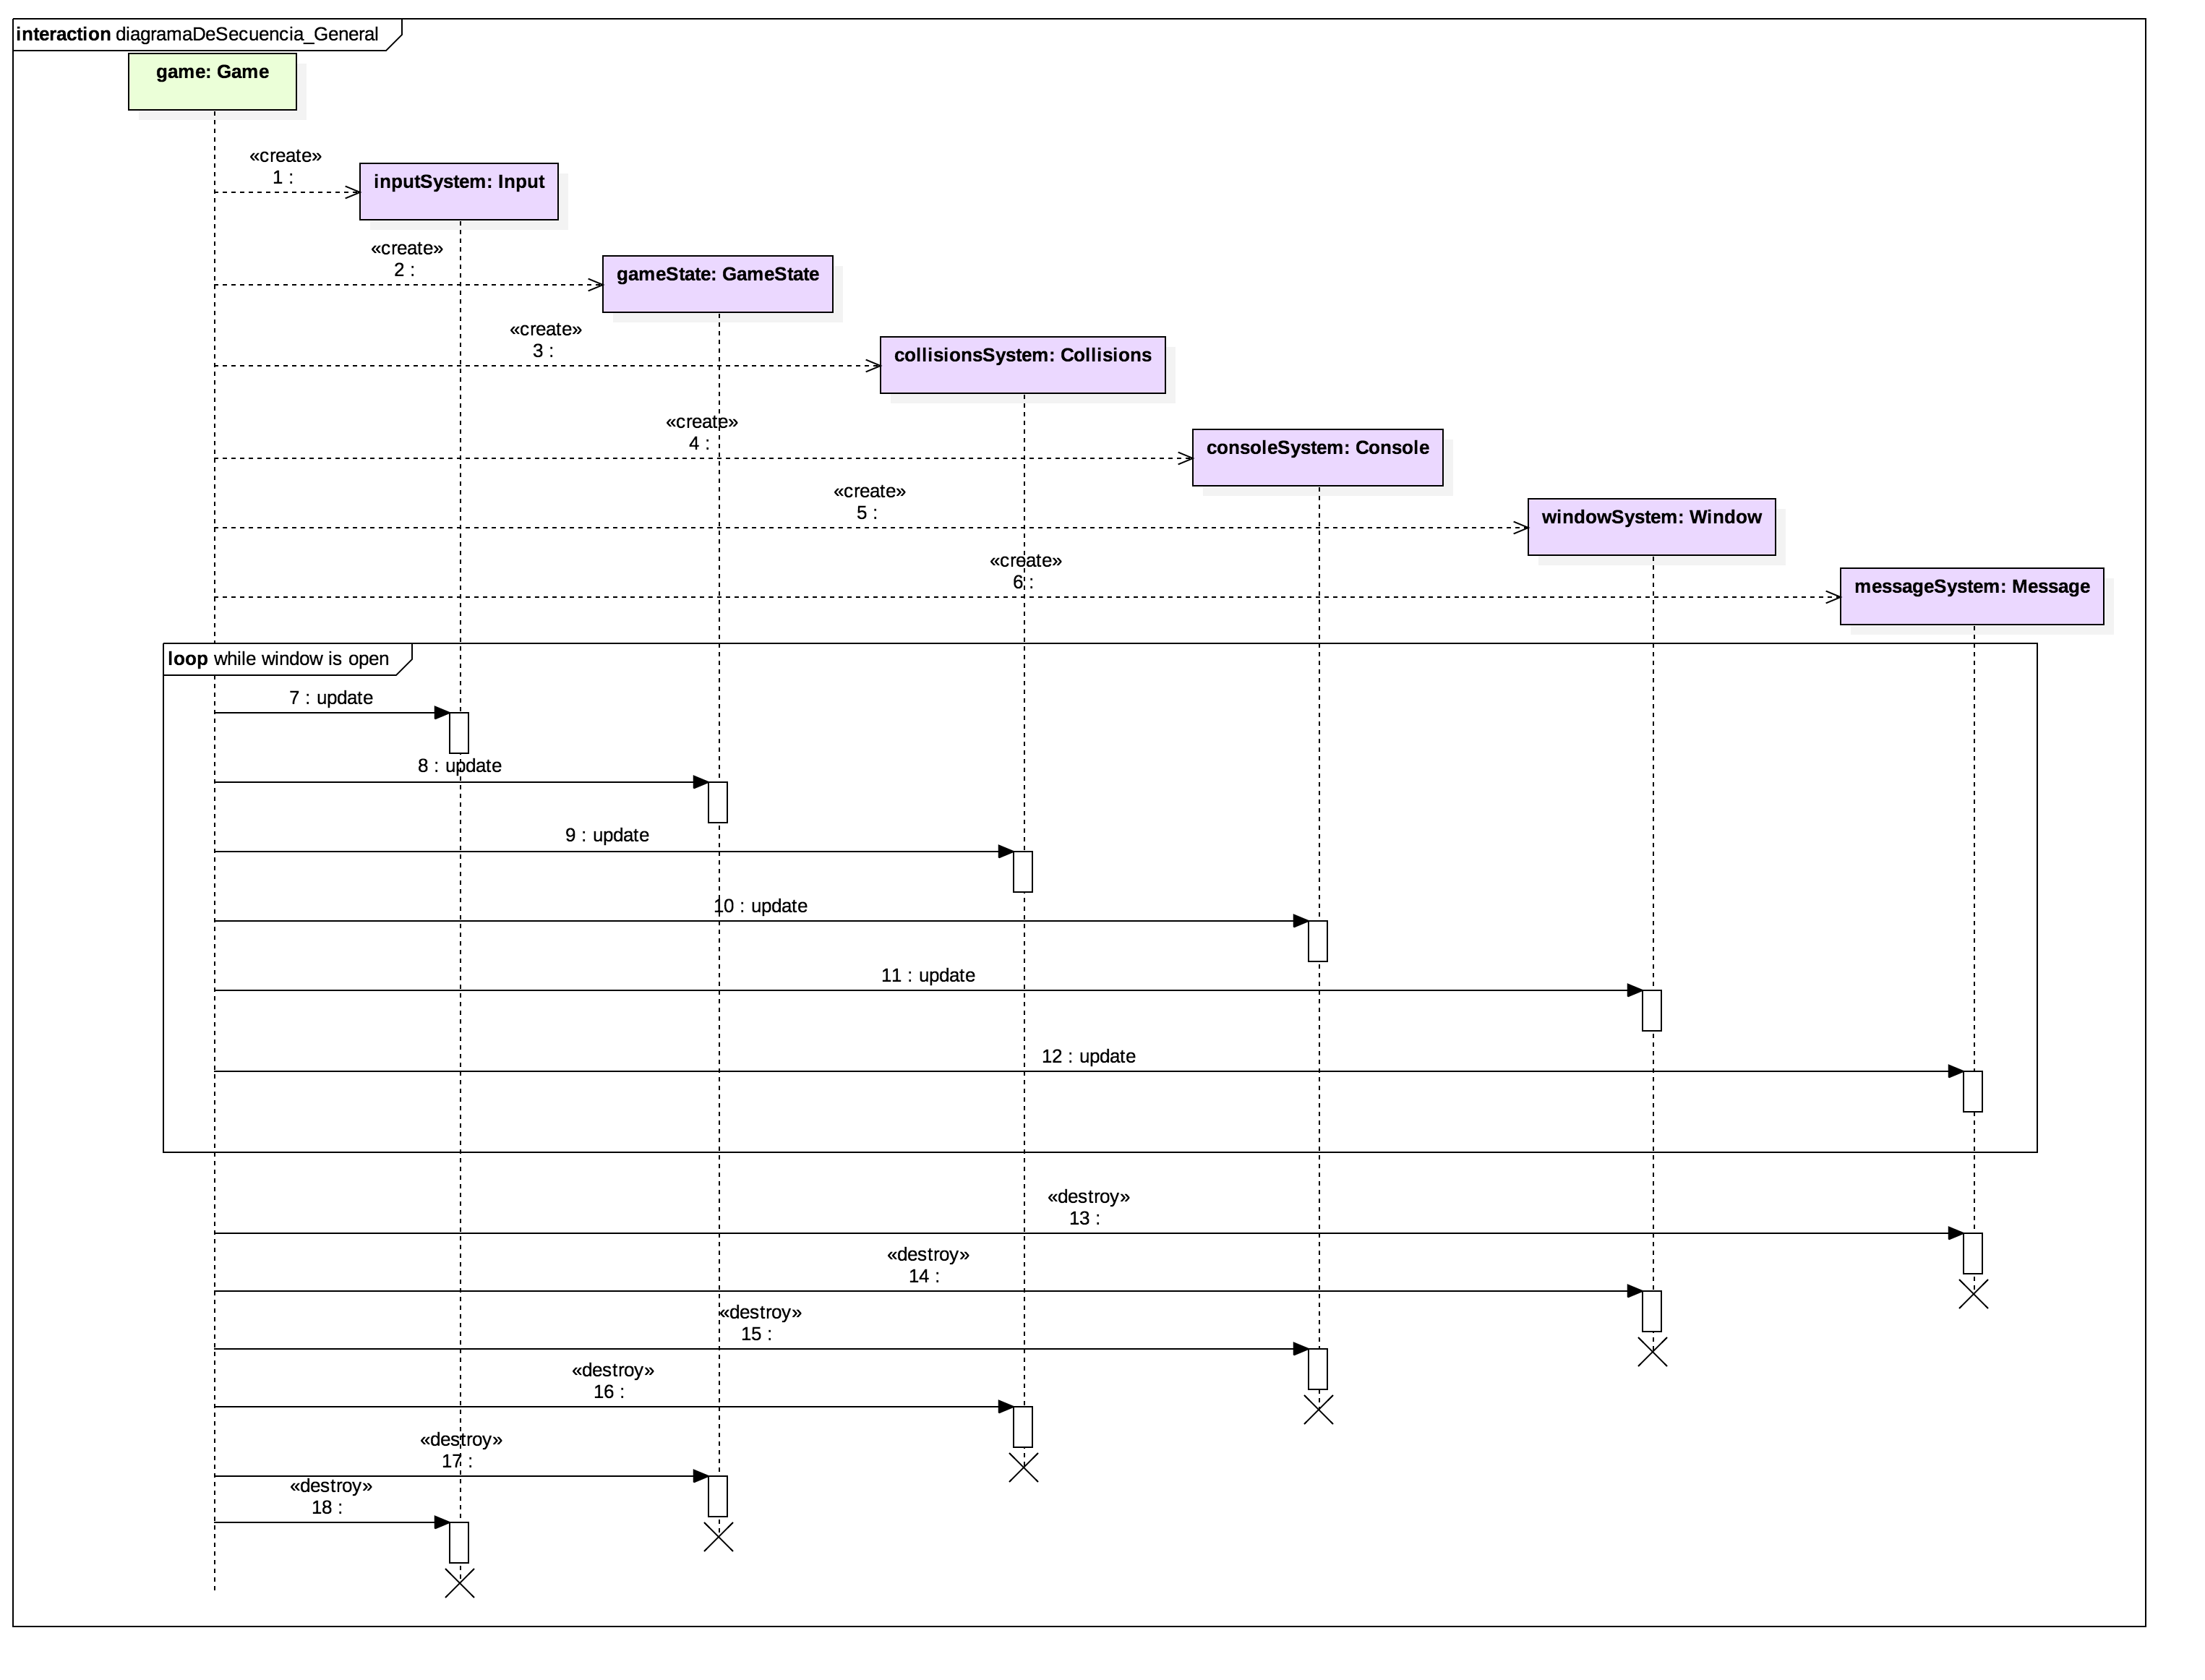
\includegraphics[width=19cm]{otros/UML/png/alld/png/CasosDeUso__General__Collaboration1__Interaction1__diagramaDeSecuencia_General_15.png}}
	\caption{Diagrama de secuencia general de la aplicación}
	\label{sec:general}
\end{figure}

La figura \ref{sec:general} muestra la creación y destrucción de los subsistemas de la aplicación, además del bucle principal del juego conocido como \textit{gameloop}. El diagrama en si mismo es sencillo, se crean todos los subsistemas y finalmente se destruyen en orden inverso.

\bigskip

El bucle contiene las actualizaciones de todas las partes de la aplicación en el mismo orden en el que se han creado aunque este podría variar. Esto podría dar lugar a pensar que el hecho de realizar el bucle en este orden de problemas en el sentido de que si un subsistema quiere modificar otro que ya ha sido actualizado, dicha modificación tiene que esperar a la siguiente iteración. De forma efectiva esto no es un problema dado que al realizar el intercambio de mensajes al final es el bus de mensajes el encargado de hacer que se ejecuten todas las funciones relacionadas con los mensajes existentes. Como mucho es posible que en algunas situaciones la ejecución de una funcionalidad se retrase una iteración pero dado que cada fotograma (y por lo tanto, cada iteración) se muestra cada unos 16 milisegundos\footnote{Contando con una frecuencia de actualización común de 60 fotogramas por segundo, que se ha probado como constante en esta aplicación en equipos relativamente actuales} no es posible que el usuario sea consciente.

\bigskip

Este diagrama se relaciona estrechamente con los casos de uso CU-1 (iniciar aplicación) y CU-2 (cerrar aplicación).

\subsubsection*{Escena genérica}

\begin{figure}
	\centerline{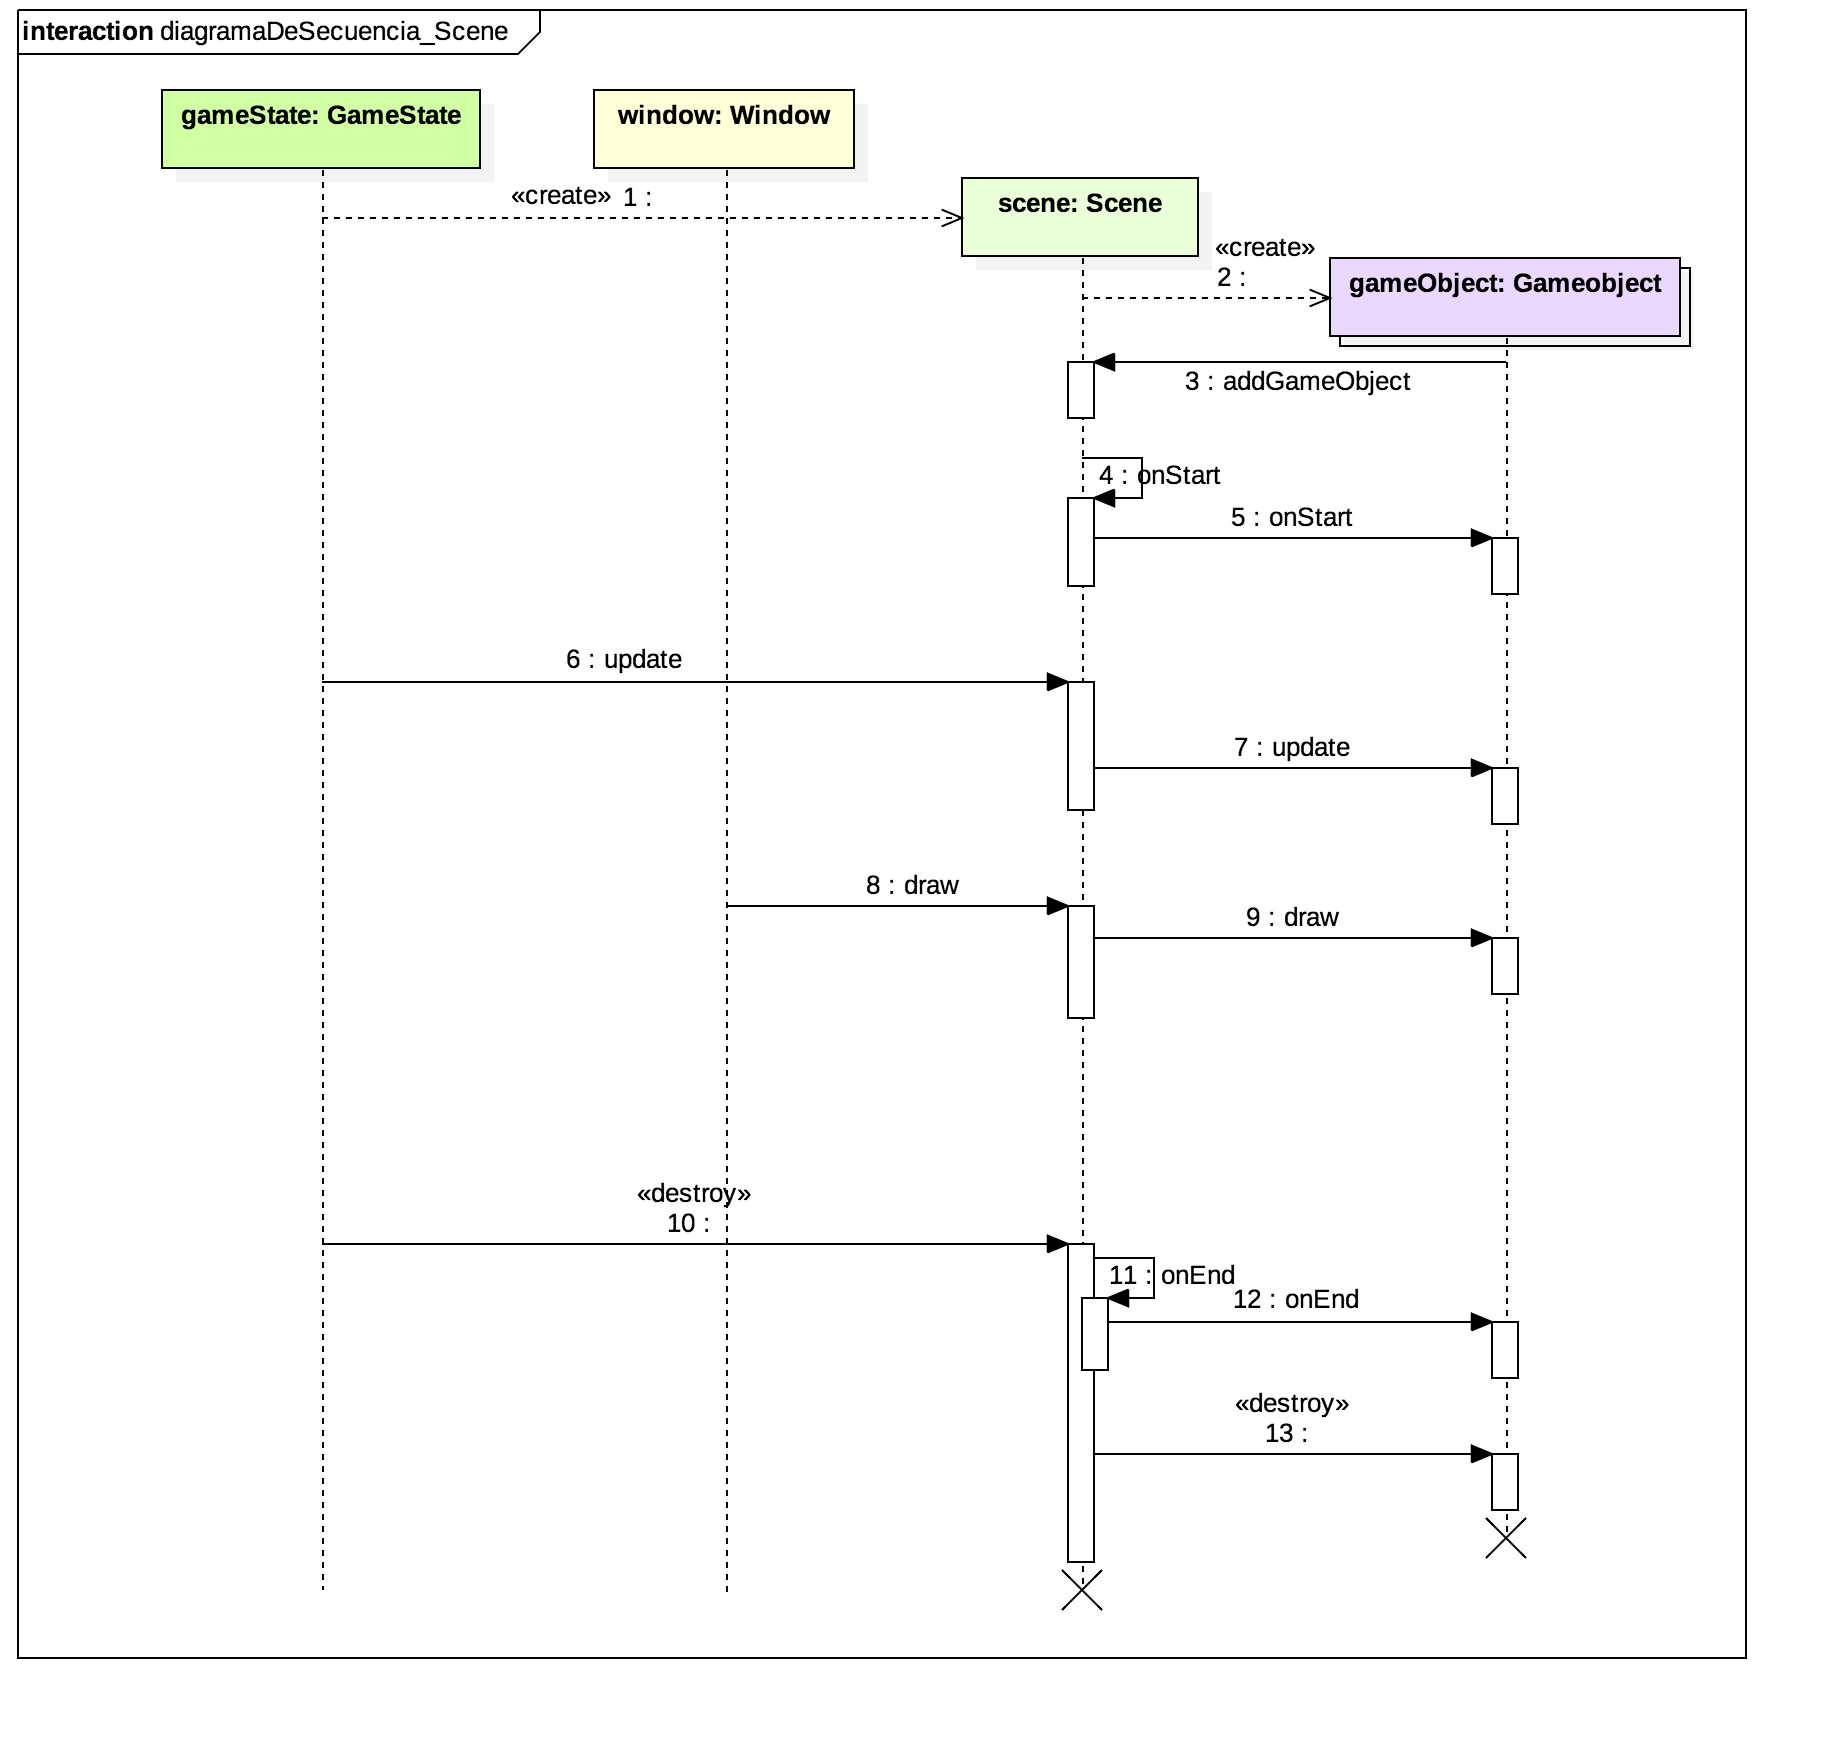
\includegraphics[width=15cm]{otros/UML/png/alld/png/CasosDeUso__General__Collaboration2__Interaction1__diagramaDeSecuencia_Scene_16.png}}
	\caption{Diagrama de secuencia genérico de una escena}
	\label{sec:scene}
\end{figure}

El diagrama de secuencia de la figura \ref{sec:scene} nos muestra cómo el objeto \textit{gameState} puede crear y destruir una escena para cambiar entre las mismas, lo que se relaciona estrechamente con el CU-3 (seleccionar y ejecutar opción). Además se muestra cómo es el \textit{gameState} el encargado de actualizar la escena pero será el subsistema de \textit{rendering} con su clase \textit{Window} el encargado de hacer que se dibuje la escena y todos sus \textit{gameobjects}.


\subsubsection*{Consola}

Relacionado estrechamente con el caso de uso CU-9 (Visualizar resultados de combates) y el requisito no funcional RNF-4 (Facilidad para depurar) está el diagrama de secuencia mostrado en la figura \ref{sec:console}.

\bigskip

En orden temporal, se muestra cómo el usuario puede introducir caracteres por teclado para crear un comando en la consola para luego ejecutarlo y que el mismo se envíe al bus de mensajes. Luego se observa cómo la clase \textit{Window}, al tener acceso a la consola, es capaz de comprobar si está abierta y dibujarla por pantalla junto con todas las lineas de texto que esta contiene.

\bigskip

Finalmente se muestra cómo el usuario puede alternar entre visualizar o no la consola al pulsar una determinada tecla interpretada por el sistema de \textit{input}.

\begin{landscape}
\begin{figure}
	\hspace*{-3cm}  
	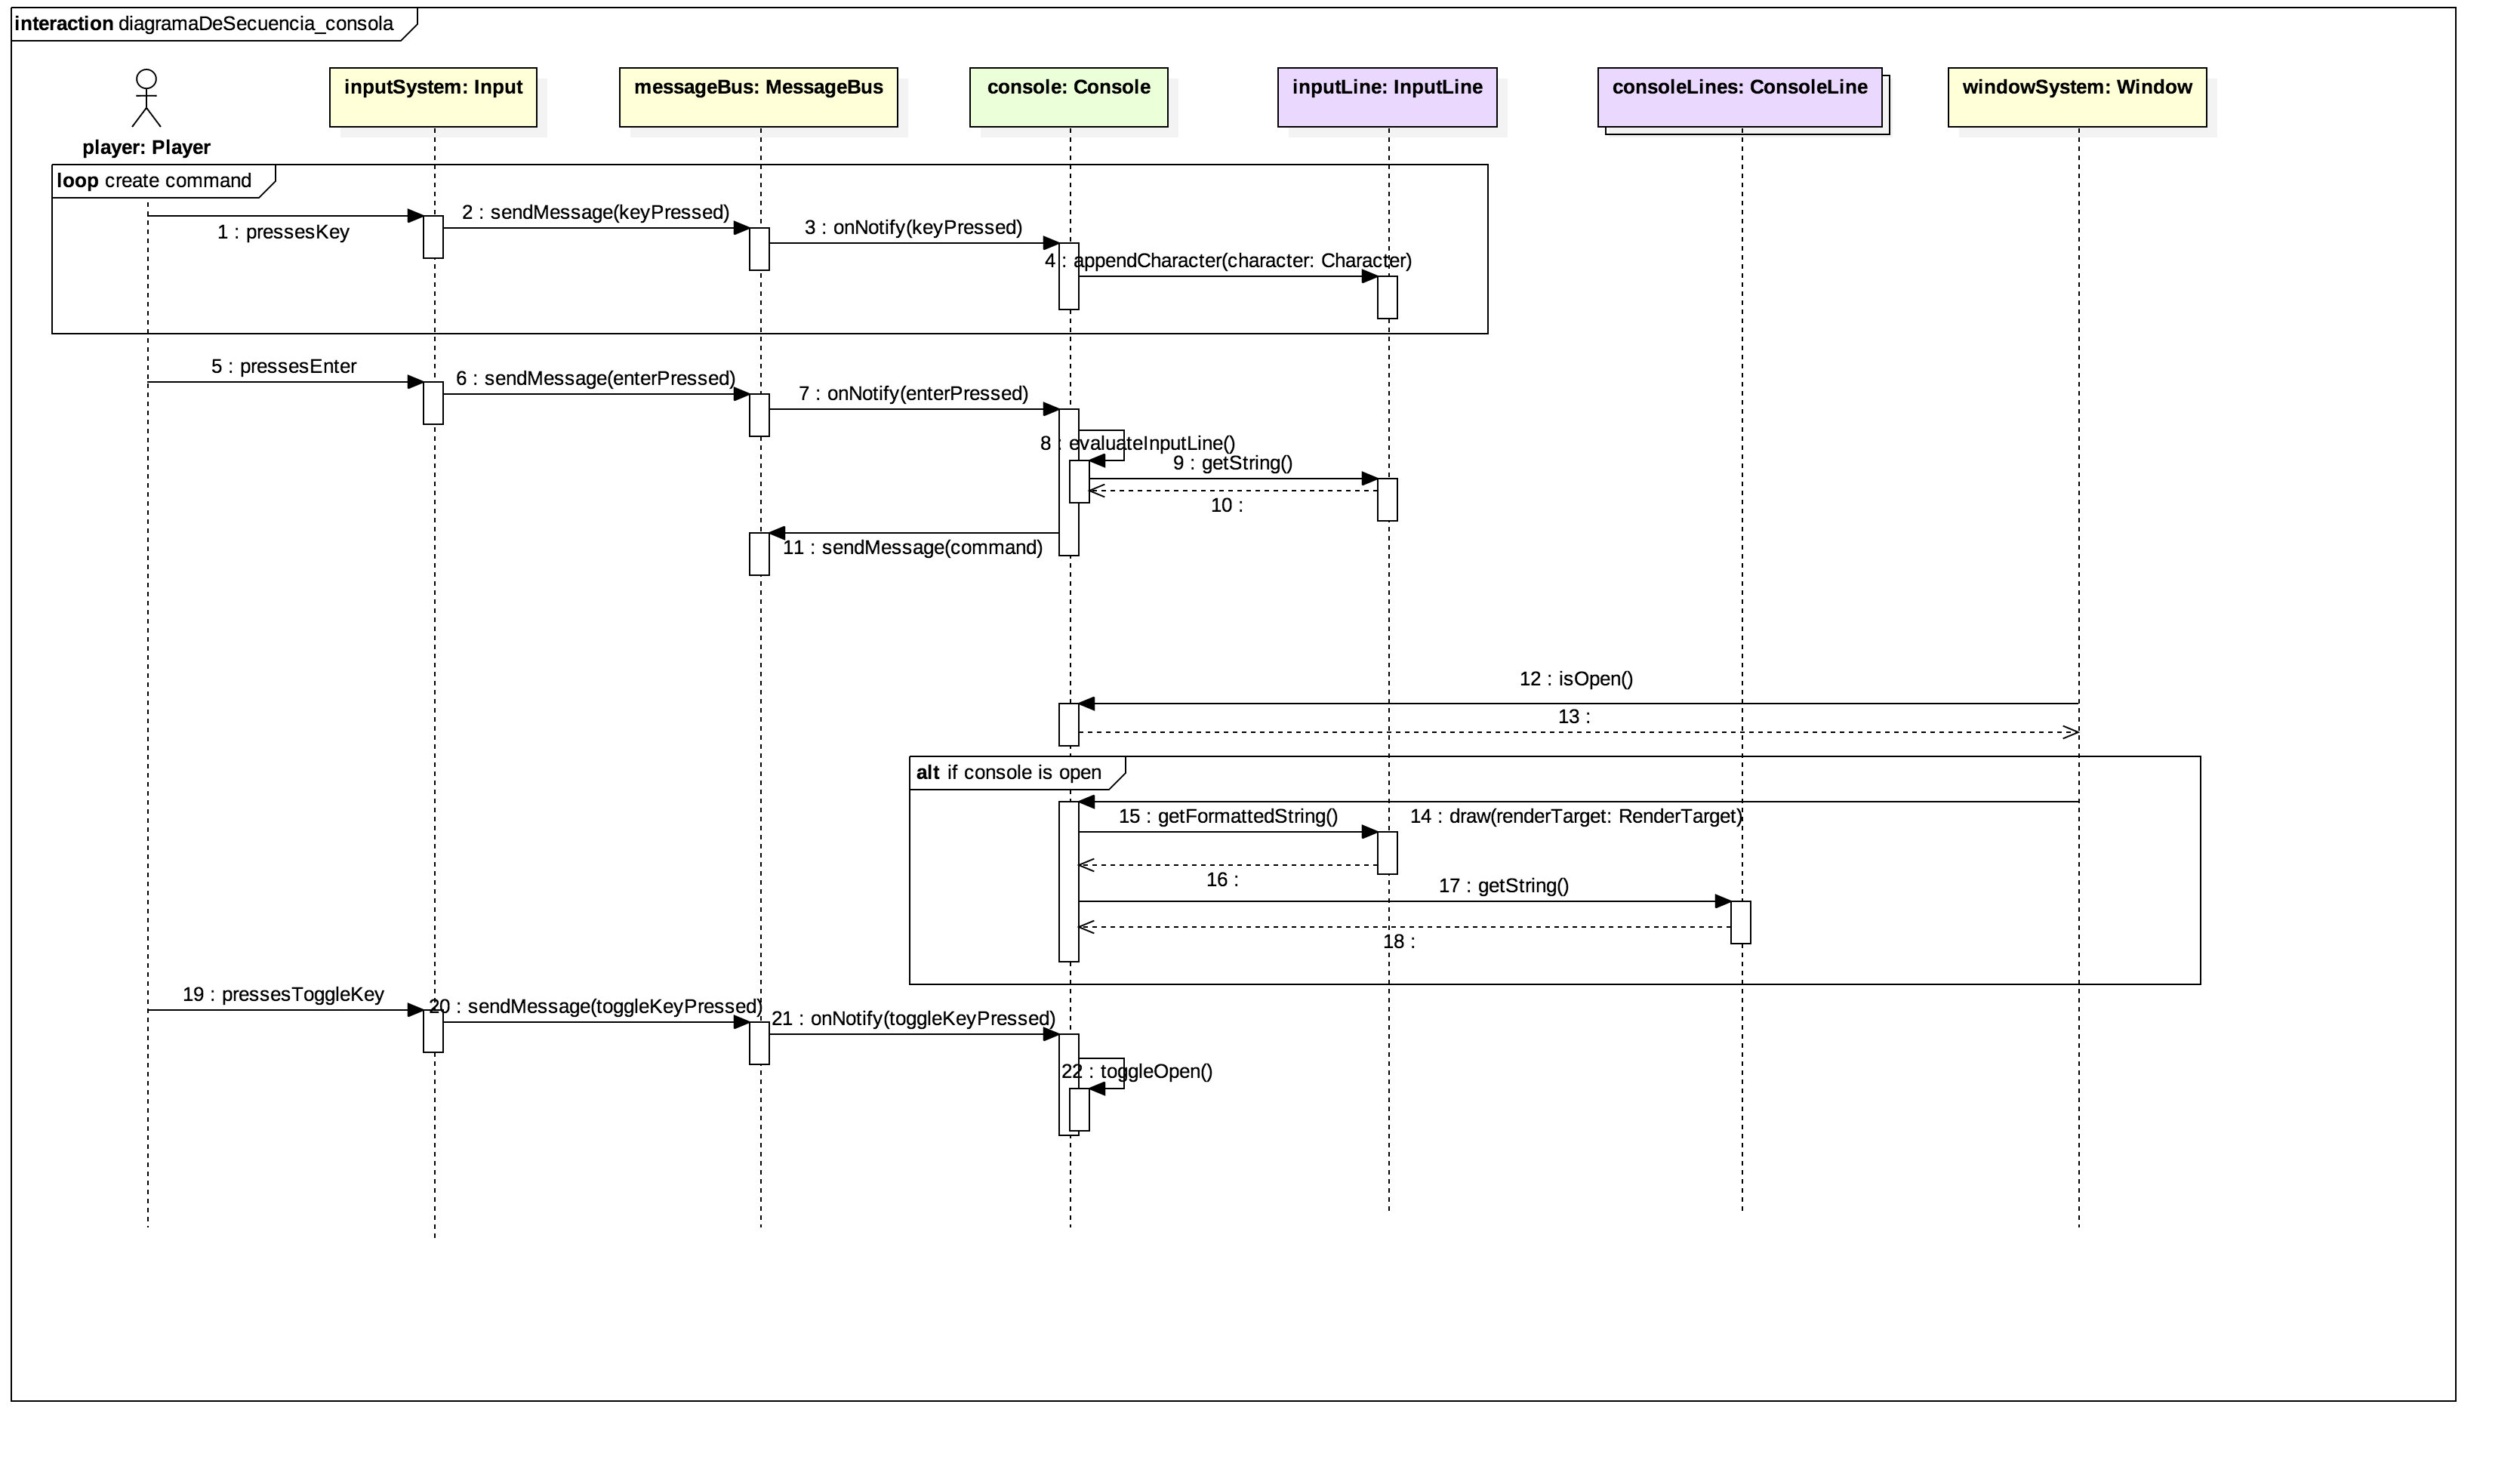
\includegraphics[width=24cm]{otros/UML/png/alld/png/CasosDeUso__Especifico__Collaboration4__Interaction1__diagramaDeSecuencia_consola_20.png}
	\caption{Diagrama de secuencia de la consola}
	\label{sec:console}
\end{figure}
\end{landscape}


\subsection{Escenas y agente}

\subsubsection*{Escena del menú}

En el diagrama de secuencia de la escena del menú de la figura \ref{sec:menu} se ve cómo el usuario es capaz de seleccionar entre las opciones del menú para luego ejecutar la seleccionada y cambiar de escena.

\bigskip

El flujo comienza por utilizar el sistema de \textit{input} para mandar mensajes referentes a cambiar la opción seleccionada. Una vez que se está en la opción deseada se envía el mensaje de ejecutar dicha opción. En este momento se envía un mensaje que llega al \textit{gameState} indicándole la nueva escena a la que habrá que cambiar, en este momento el \textit{gameState} destruye la escena del menú y genera la nueva escena según la opción seleccionada.

\begin{landscape}
\begin{figure}
	\hspace*{-3cm}  
	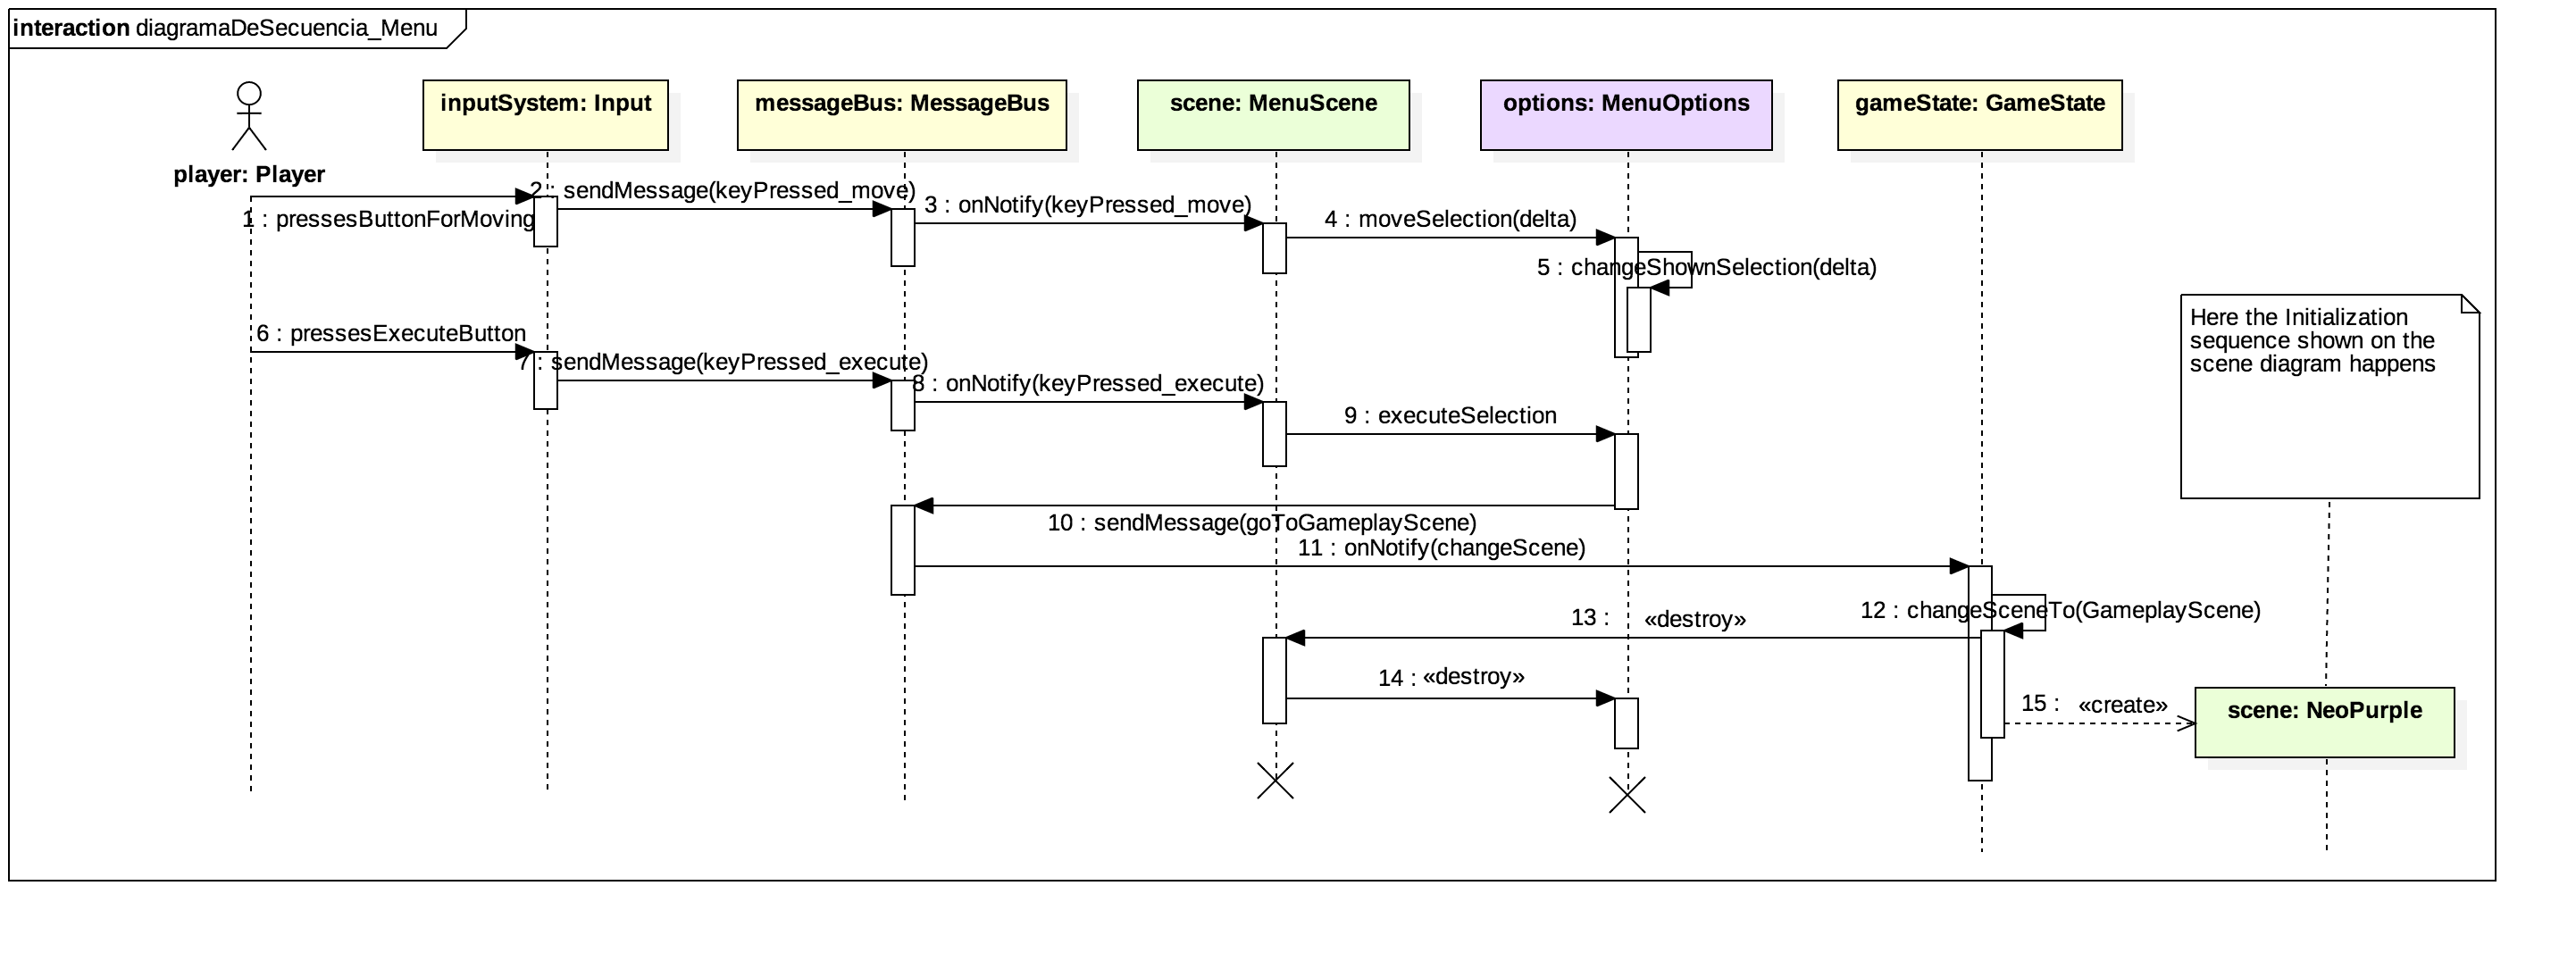
\includegraphics[width=24cm]{otros/UML/png/alld/png/CasosDeUso__Especifico__Collaboration1__Interaction1__diagramaDeSecuencia_Menu_17.png}
	\caption{Diagrama de secuencia de la escena del menú}
	\label{sec:menu}
\end{figure}
\end{landscape}

\subsubsection*{Escena del juego}

La figura \ref{sec:gameplay} contiene el diagrama de secuencia que indica la interacción de un jugador con el videojuego, relacionado con los casos de uso CU-7 (jugador contra agente) y CU-8 (jugador contra jugador).

\bigskip

En el diagrama se muestra cómo el jugador realiza todas las acciones disponibles para el durante un combate en el siguiente orden temporal:

\begin{enumerate}
	\item El jugador mueve el \textit{joystick} del mando y el mismo se traduce en su personaje moviéndose por la escena.
	\item El jugador pulsa el botón de atacar en el mando y su personaje realiza un ataque.
	\item El jugador pulsa el botón de defenderse y su personaje hace lo propio.
	\item El jugador pulsa el botón de volver al menú, el combate y la escena terminan y se vuelve a la escena del menú.
\end{enumerate}

\begin{figure}
	\centerline{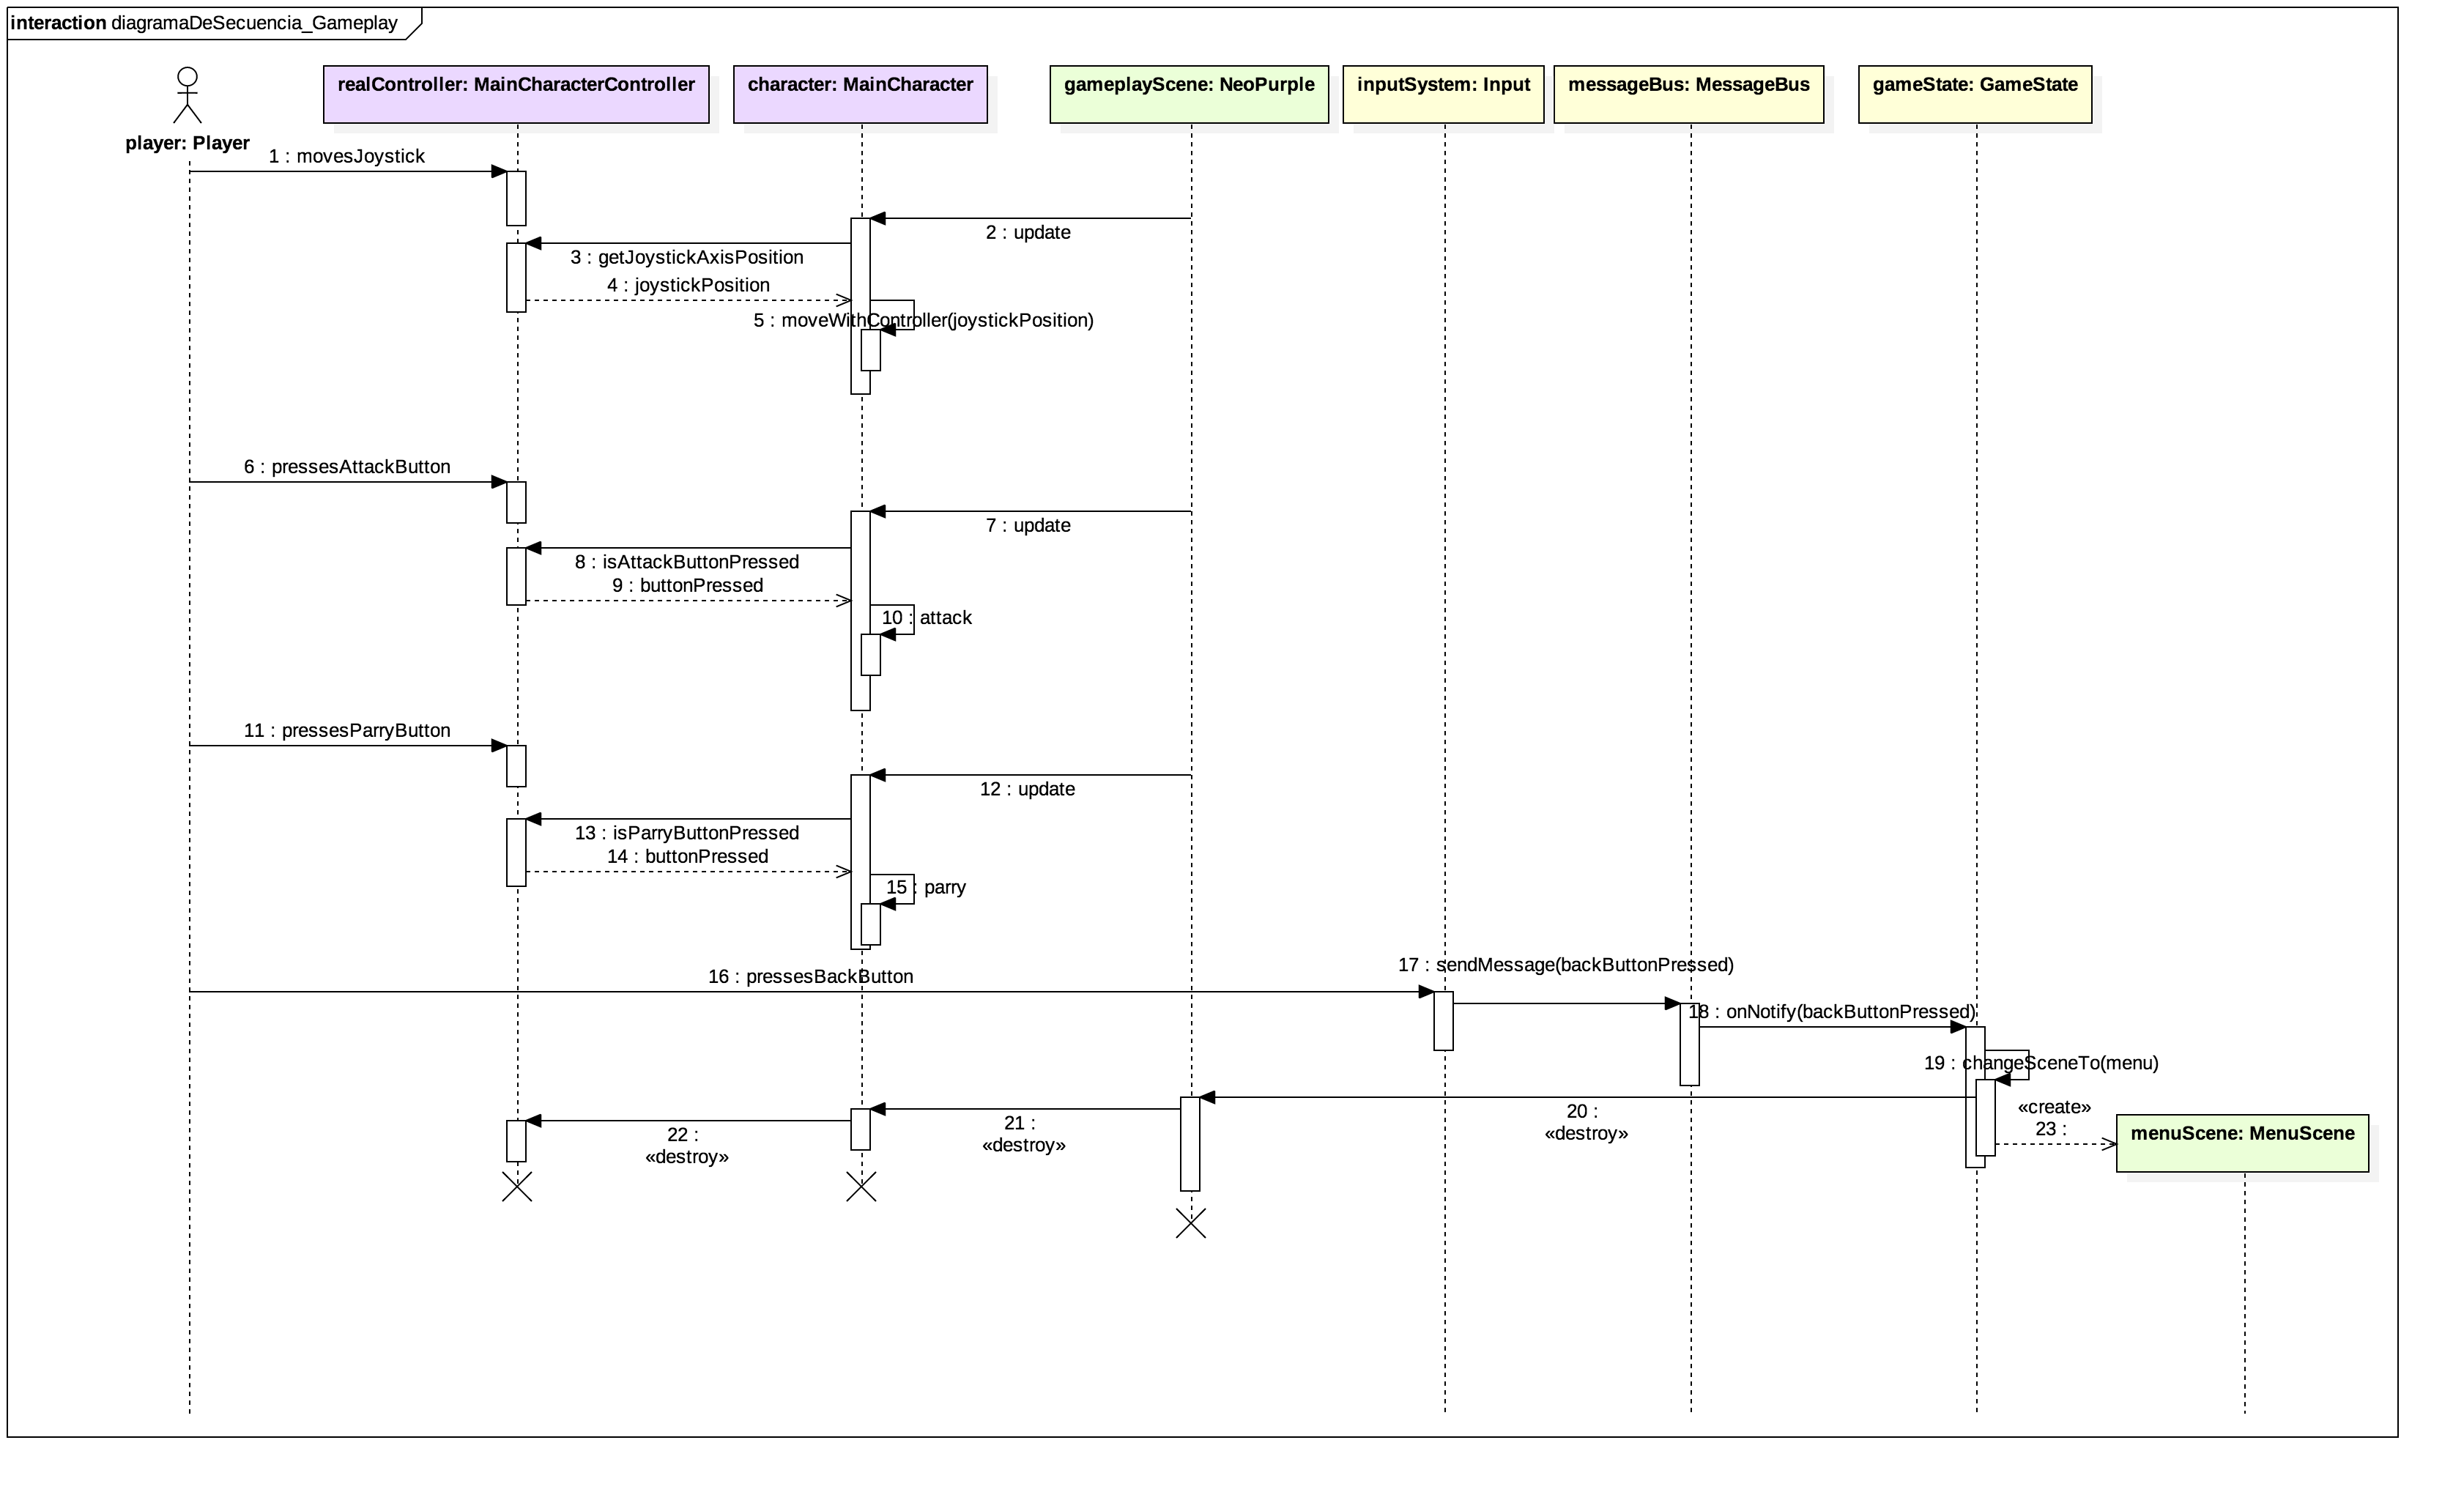
\includegraphics[width=19cm]{otros/UML/png/alld/png/CasosDeUso__Especifico__Collaboration2__Interaction1__diagramaDeSecuencia_Gameplay_18.png}}
	\caption{Diagrama de secuencia de la escena del \textit{gameplay}}
	\label{sec:gameplay}
\end{figure}


\subsubsection*{Agente}


Finalmente, la figura \ref{sec:agent} contiene el diagrama de secuencia asociado al agente y sus acciones. Será más sencillo comprenderlo al relacionarlo con el diagrama de clases del agente mostrado en la figura \ref{class:agent}. Para explicar la secuencia de pasos que se están dando se hace uso de la siguiente enumeración:

\begin{enumerate}
	\item La escena actualiza al agente y este hace lo mismo con su \textit{Observer}.
	\item El comportamiento (\textit{Behaviour}) se actualiza y discretiza el estado continuo mediante el uso del \textit{Observer}.
	\item Se actualiza el conocimiento del agente enviando los datos al \textit{StateActionContainer} y se obtiene del mismo el conocimiento previo sobre el estado actual.
	\item Se calcula la acción a llevar a cabo y se ejecuta con la ayuda de \textit{Actions}. Este objeto modificará el \textit{controller} con los parámetros adecuados.
	\item El personaje leerá los datos del \textit{controller} y ejecutará una de las acciones según el estado de este mando virtual.
\end{enumerate}

\begin{figure}
	\centerline{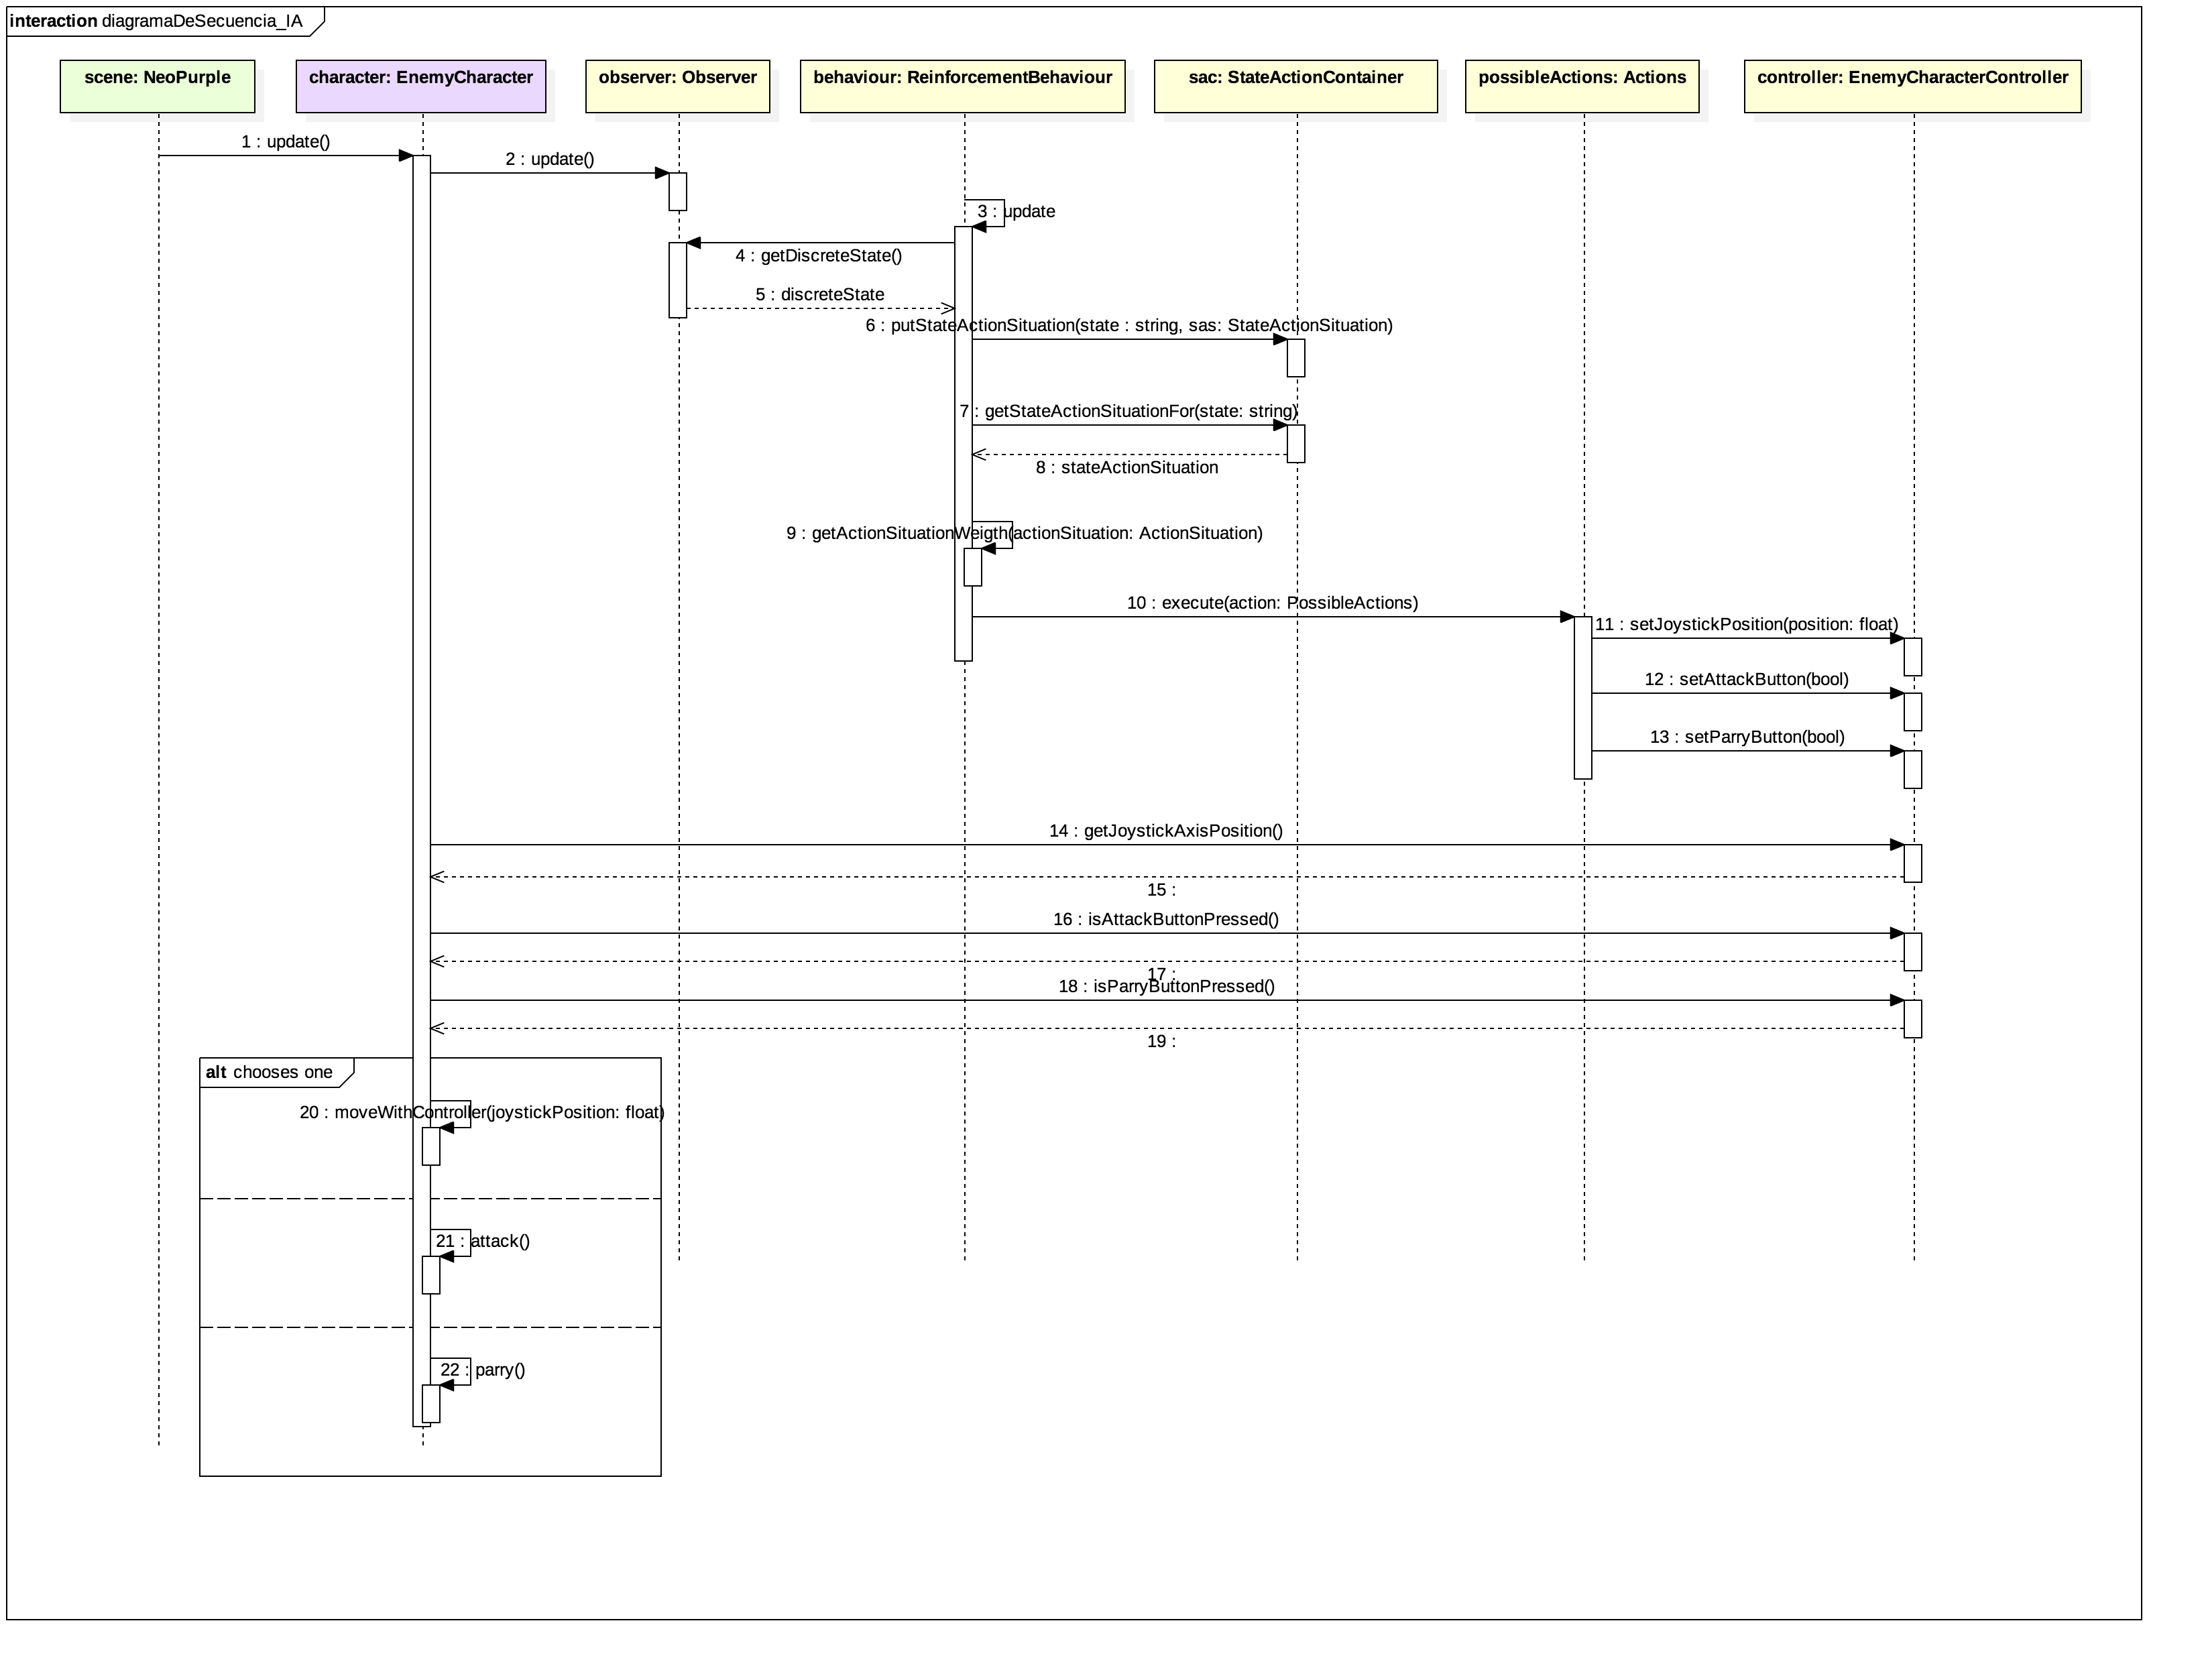
\includegraphics[width=19cm]{otros/UML/png/alld/png/CasosDeUso__Especifico__Collaboration3__Interaction1__diagramaDeSecuencia_IA_19.png}}
	\caption{Diagrama de secuencia del agente}
	\label{sec:agent}
\end{figure}

\section{Diseño de la interfaz gráfica}

Este apartado muestra los diseños realizados primero en papel en referencia a la interfaz gráfica de la aplicación. Dichos diseños son sencillos ya que a diferencia de aplicaciones de otros tipos, los videojuegos de este género suelen optar por evitar una gran cantidad de opciones en una misma vista tendiendo normalmente al minimalismo.

\bigskip

La ventana tendrá una relación de aspecto constante de 4:3 para evocar un parecido con videojuegos antiguos que utilizaban una relación similar dados los estándares de los televisores de la época. Esto debería favorecer la comodidad y dar un aspecto general familiar a los usuarios.

\bigskip

En relación con el requisito no funcional RNF-8 (referente a la usabilidad de la aplicación) se ha buscado la máxima comodidad a la hora de controlar el juego mediante el uso de un mando. Por ello, todos los controles, tanto del menú como del combate están enfocados a ser realizados con un mando similar al de una videoconsola, dejando a un lado el uso del teclado solamente para funciones de depuración o avanzadas tales como abrir y escribir en la consola.

\bigskip

Otro aspecto muy relacionado con la usabilidad es el uso de un indicador sonoro a todas las acciones importantes que se realizan. Dicho indicador tiene que ser constante con la acción que se está mostrando en la interfaz.

\subsection{Interfaz del menú}

En el \textit{mockup}\footnote{Modelo de diseño de una interfaz que permite realizar cambios a la misma sin necesidad de implementarla y con el fin de evaluar a grandes rasgos su usabilidad y aspecto} del menú mostrado en la figura \ref{inter:menu} se vé cómo se ha echo hincapié en la simplicidad del mismo. El título se muestra utilizando un tamaño de fuente superior y las opciones se alinean por la izquierda teniendo en cuenta que pueden tener una longitud distinta.

\bigskip

La opción seleccionada se muestra en negrita y subrayada para no dar lugar a dudas a la hora de distinguirla de las otras. Tanto el cambio entre opciones como la ejecución de una de ellas tienen un sonido asociado lo suficientemente diferente como para ser inconfundibles entre ellos.

\bigskip A la hora de colocar el título y las opciones se ha utilizado la conocida como regla de los tercios\footnote{Regla, generalmente asociada a la fotografía, que sugiere que alinear vertical y horizontalmente los elementos de una fotografía con las líneas imaginarias que separa la imagen en tercios las hace más interesantes, naturas y cómodas a la vista}

\begin{figure}
	\centerline{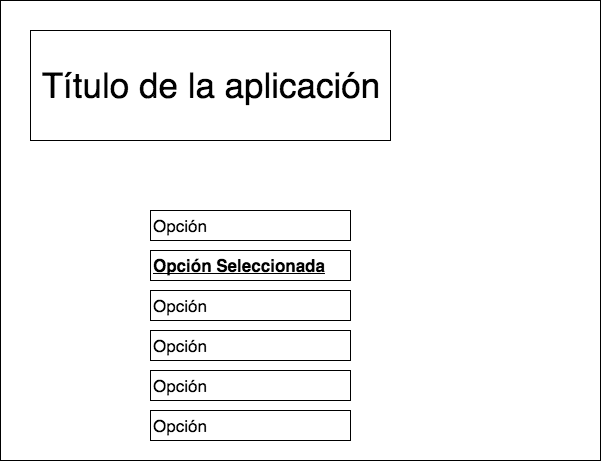
\includegraphics[width=12cm]{otros/graphicalInterface/menu.png}}
	\caption{\textit{Mockup} de la interfaz del menú}
	\label{inter:menu}
\end{figure}

\subsection{Interfaz del combate}

La figura \ref{inter:combat} contiene el \textit{mockup} de la interfaz que el usuario ve al realizar el combate entre personajes. En el mismo se distinguen dos partes diferenciadas:

\bigskip

En la parte superior de la pantalla se ven las barras de vida de los personajes identificadas por colores, dichas barras de vida decrecerán en tamaño horizontalmente para indicar que el personaje asociado ha recibido daño. En el centro se ve un número que indica los segundos restantes del combate, cuando dicho contador llega a cero se termina el combate y gana el jugador con más vida, empatando si es igual. Este tipo de interfaz de combate pretende recordar a la empleada por antiguos juegos de peleas 2D en recreativas tales como \textit{Street Fighter} o \textit{Mortal Kombat} lo que ayuda a que el usuario la considere familiar.

\bigskip

En el centro de la pantalla se puede ver claramente la zona de combate con ambos personajes. Dicha zona se diferencia del resto de la pantalla al utilizar un fondo completamente negro haciendo sencillo el hecho de darse cuenta de que la zona en la que se pueden mover los personajes está limitada. Además los personajes cuentan con un indicador por colores que los relacionan con sus barras de vida para facilitar su identificación durante la batalla.

\bigskip

Durante el combate el hecho de atacar producirá un sonido específico, de la misma forma que recibir daño. Esto incrementa la familiarización del jugador ya que combina la animación mostrada y el sonido con la acción que acaba de ocurrir.

\bigskip

Pese a que no se muestre en la figura, cuando se detiene el combate porque uno de los personajes ha derrotado al otro se muestran letras que indican el jugador ganador, ocupando las mismas toda la pantalla y siendo dibujadas con el mismo color que identifica a cada personaje.

\begin{figure}
	\centerline{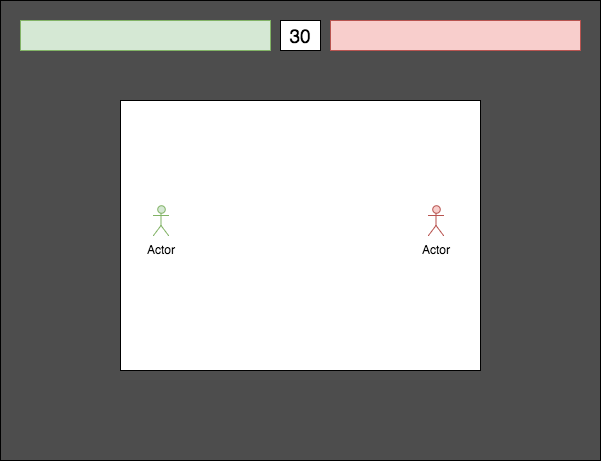
\includegraphics[width=12cm]{otros/graphicalInterface/gameplay.png}}
	\caption{\textit{Mockup} de la interfaz del combate}
	\label{inter:combat}
\end{figure}

\subsection{Interfaz de la consola}

Finalmente, la figura \ref{inter:console} muestra cómo se vería la consola sobre la aplicación. Recordemos que la misma se puede abrir y cerrar en cualquier escena por lo que tiene un fondo coloreado pero que cierta transparencia que permita ver fácilmente lo que está ocurriendo.

\bigskip

Al fondo de la consola se puede observar una línea con el símbolo $>$ que identifica a la línea de entrada para el usuario. SI la consola está abierta y se escribe en el teclado los caracteres se agregarán a esta línea, siendo limpiada al pulsar \textit{intro}. Las líneas en un negro ligeramente más suave situadas por encima representan los mensajes relevantes que la consola está mostrando al usuario. Finalmente, en la esquina superior izquierda se puede ver un contador de fotogramas por segundo o \textit{FPS}.

\begin{figure}
	\centerline{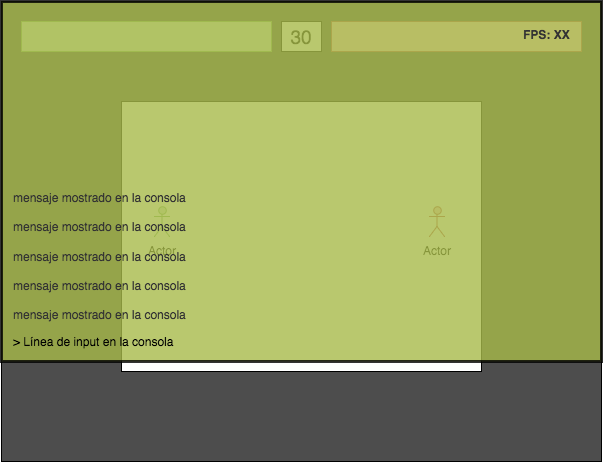
\includegraphics[width=12cm]{otros/graphicalInterface/console.png}}
	\caption{\textit{Mockup} de la interfaz de la consola}
	\label{inter:console}
\end{figure}


